\section[Introduction]{Introduction \& Research Objectives}

% Section transition: 01_INTRODUCTION_AND_RESEARCH_OBJECTIVES
\IceSectionDivider{}{Introduction\\ \&\\ Research Objectives}{FIGURES/SECTION_TRANSITION/ICE_WING.jpg}


% ---------------------------------------------------------------------------
% Slide 1: Aircraft Icing: Context and Motivation
% ---------------------------------------------------------------------------
\begin{frame}{Aircraft Icing: Context and Motivation}

\vspace{0.15cm}

\begin{columns}[T,onlytextwidth]
\hspace*{\fill}%
% LEFT COLUMN
\begin{column}{0.41\textwidth}
\justifying

\vspace{0.3cm}

{\small Aircraft manufacturers strive to develop
\textbf{\color{champsBlue}lighter and more
efficient aircraft}, while ensuring
\textbf{safe operation} under a wide range
of atmospheric conditions.}

\vspace{0.2cm}

{\small Among these challenges,
\textbf{\color{champsBlue}in-flight icing}\\
remains a major concern.}

\end{column}
\hspace{0.5cm}%
% RIGHT COLUMN
\begin{column}{5.5cm}

\begin{tikzpicture}
  \begin{scope}
    \clip[rounded corners=5pt]
        (0,0) rectangle (5.5,2.75);

    \node[inner sep=0pt] at (2.25,1.375) {
        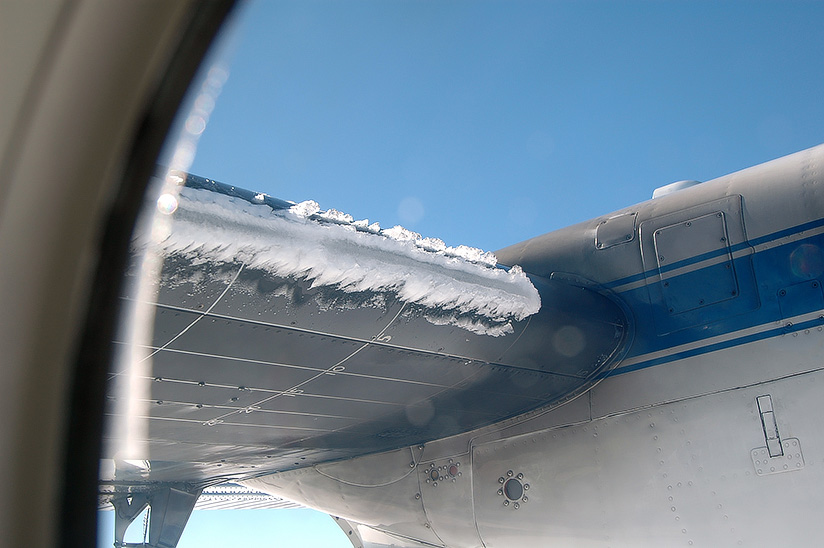
\includegraphics[
            width=6.8cm
        ]{FIGURES/SECTION_TRANSITION/ICE_WING.jpg}
    };
  \end{scope}
    \node[anchor=north,inner sep=0pt,font=\scriptsize,text=gray]
        at (2.75,-0.15) {Ice accretion on an aircraft wing*.};
\end{tikzpicture}

\end{column}
\hspace*{\fill}%

\end{columns}

\vspace{0.15cm}

% BOTTOM PHYSICAL PROCESS
\begin{center}
\vspace{-0.2cm}
\begin{tikzpicture}

\node[
    fill=champsBlue!7,
    rounded corners=4pt,
    text width=0.9\textwidth+0.4cm,
    inner xsep=0.05cm, inner ysep=0.25cm,
    align=center
] {
    \textbf{\color{champsBlue}
    Supercooled droplets}
    freeze and accumulate on aircraft surfaces,\\
    altering their geometry and aerodynamic behavior.
};

\end{tikzpicture}
\end{center}

\vspace{-0.1cm}

\begin{columns}[T,onlytextwidth]

\begin{column}{0.48\textwidth}
\centering
{\color{champsBlue}\bfseries
Aerodynamic Performance Loss}

\vspace{0.08cm}
{\small Increased drag, reduced lift,\\
and degraded handling qualities}
\end{column}

\begin{column}{0.48\textwidth}
\centering
{\color{champsBlue}\bfseries
Flight Safety Risks}

\vspace{0.08cm}
{\small\justifying Potential loss of control
and catastrophic accidents}
\end{column}

\end{columns}

\begin{tikzpicture}[remember picture,overlay]
  \node[anchor=south west,font=\tiny,text=gray]
      at ([xshift=0.1cm,yshift=0.27cm]current page.south west)
      {*Image from Flight Society Foundation\quad\cite{CAO2018353,lynch2001effects,cao2015aircraft}};
\end{tikzpicture}

\end{frame}

% ---------------------------------------------------------------------------
% Slide 2: Aircraft Icing: Prediction and Certification
% ---------------------------------------------------------------------------
\begin{frame}{Aircraft Icing: Prediction and Certification}

\vspace{-0.15cm}

\noindent\resizebox{\textwidth}{!}{Accurate assessment of aircraft icing
is essential to demonstrate safe operation
under icing conditions.}

\vspace{0.05cm}
\vspace{0.25cm}
{\centering\color{champsBlue}\bfseries\large Three Complementary Approaches\par}
\vspace{0.1cm}

\vspace{-0.05cm}

\begin{columns}[T,onlytextwidth]

% FLIGHT TESTS
\begin{column}{0.32\textwidth}
\introCard
    {}
    {In-Flight Testing}
    {
    \textbf{Realistic operating conditions}

    \vspace{0.1cm}

    \textcolor{red!70!black}{\textbf{Limitations:}}

    High costs, safety risks, and
    limited control over atmospheric
    conditions.
    }
\end{column}

% WIND TUNNEL
\begin{column}{0.32\textwidth}
\introCard
    {}
    {Wind Tunnel Testing}
    {
    \textbf{Controlled experimental conditions}

    \vspace{0.1cm}

    \textcolor{red!70!black}{\textbf{Limitations:}}

    Scaling difficulties, facility
    constraints, and significant
    experimental costs.
    }
\end{column}

% NUMERICAL
\begin{column}{0.32\textwidth}
\introCard
    {}
    {Numerical Simulations}
    {
    \textbf{Flexible and cost-effective prediction}

    \vspace{0.1cm}

    \textcolor{champsBlue}{\textbf{Opportunities:}}

    Wider exploration of icing
    conditions and a growing role
    in certification activities.
    }
\end{column}

\end{columns}

\vspace{0.1cm}

\begin{center}
\begin{tikzpicture}
\node[fill=champsBlue!8, rounded corners=4pt,
      text width=0.88\textwidth, inner sep=6pt,
      align=center, font=\small] {%
\textbf{\color{champsBlue}
Numerical simulations complement experimental
testing and\\ motivate the development of
accurate, robust ice-accretion frameworks.}
};
\end{tikzpicture}
\end{center}

\SlideRef{FAAAppendixC,FAAAppendixO,potapczuk2013aircraft,wright2008user}
\end{frame}

% ---------------------------------------------------------
% Separation of physical time scales
% ---------------------------------------------------------
\begin{frame}{Separation of Physical Time Scales}

\vspace{0.1cm}

\noindent\resizebox{\textwidth}{!}{Aircraft icing involves physical processes operating
at significantly different characteristic time scales.}

\vspace{0.15cm}

\begin{center}
\begin{tikzpicture}
\node[fill=champsBlue!7, rounded corners=4pt, inner xsep=0.5cm, inner ysep=0.2cm] {%
{\Large
$\displaystyle
\tau_{\mathrm{flow}},
\quad \tau_{\mathrm{droplet}}
\ \ll\
\tau_{\mathrm{ice}}
$}};
\end{tikzpicture}

\vspace{0.7cm}
$\displaystyle
\tau_{\mathrm{flow}}=\frac{L}{U_\infty}\sim\mathcal{O}(10^{-2}\,\mathrm{s}),\qquad
\tau_{\mathrm{droplet}}=\frac{\rho_d D^2}{18\mu_a}\sim\mathcal{O}(10^{-3}\,\mathrm{s}),\qquad
\tau_{\mathrm{ice}}=\frac{L}{V_{\mathrm{ice}}}\sim\mathcal{O}(10^{5}\,\mathrm{s})$
\end{center}

\vspace{0.2cm}

\begin{center}
\begin{tikzpicture}
\node[
    fill=champsBlue!7,
    rounded corners=4pt,
    text width=0.9\textwidth,
    inner sep=0.25cm,
    align=justify
] {
    \centering{\color{champsBlue}\bfseries Quasi-Steady Hypothesis}\\[0.1cm]\justifying
    The airflow and droplet-impingement solutions are
    assumed steady during each ice-accretion interval,
    with the geometry updated between successive intervals.
};
\end{tikzpicture}
\end{center}

\SlideRef{guardoneReview}
\end{frame}

% ---------------------------------------------------------
% Quasi-steady ice-accretion workflow
% ---------------------------------------------------------
\begin{frame}{Numerical Ice-Accretion Modeling}

\begin{columns}[c,onlytextwidth]

% LEFT: steps, highlighted one at a time
\begin{column}{0.58\textwidth}
\IcingText{01 \quad Geometry and Mesh Representation}
{Definition of the initial geometry using
a \textbf{body-fitted} or
\textbf{immersed-boundary} approach.}\par\vspace{0.22cm}
\IcingText{02 \quad Aerodynamic Flow}
{Air velocity $\mathbf{u}_a$, pressure $p$,
temperature $T$, and heat-transfer
coefficient (HTC).}\par\vspace{0.22cm}
\IcingText{03 \quad Droplet Impingement}
{Droplet trajectories and collection
efficiency $\beta$, yielding the
impinging water mass flux
$\dot{m}_{\mathrm{imp}}$.}\par\vspace{0.22cm}
\IcingText{04 \quad Thermodynamics and Ice Growth}
{Surface mass and energy balances
yielding the ice accretion rate
$\dot{m}_{\mathrm{ice}}$ and
ice thickness $h_{\mathrm{ice}}$.}\par\vspace{0.22cm}
\IcingText{05 \quad Geometry and Mesh Update}
{Update the ice geometry and adapt
the computational representation
for the next accretion step.}
\end{column}

% RIGHT: one image at a time, centred
\begin{column}{0.40\textwidth}
\centering
\only<1>{%
  {\scriptsize\color{champsBlue}\bfseries Body-fitted}\par\vspace{0.05cm}
  {\setlength{\fboxsep}{0pt}\setlength{\fboxrule}{0.6pt}\fbox{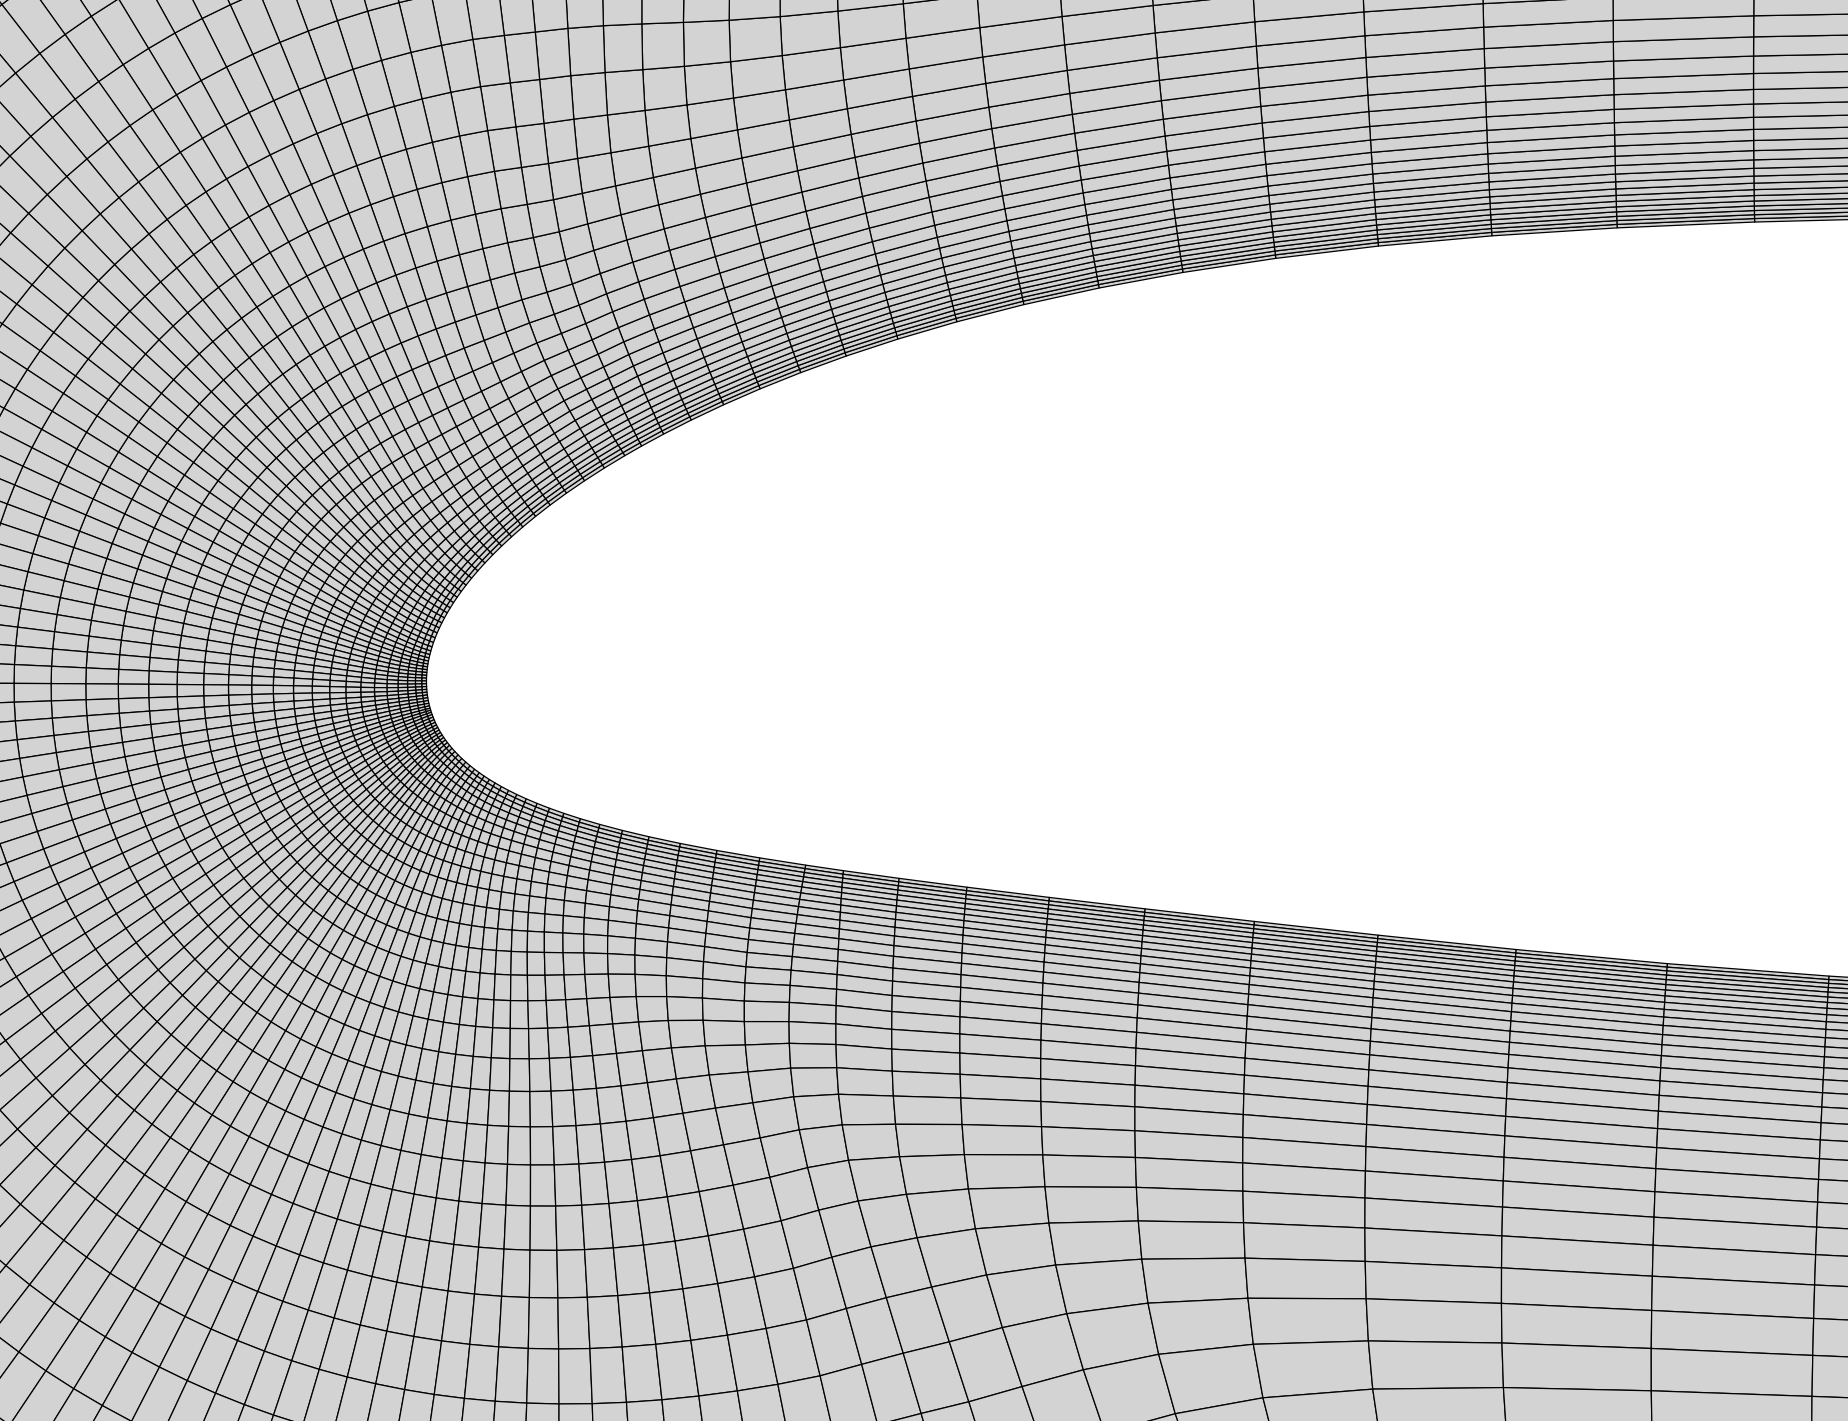
\includegraphics[width=\linewidth,height=2.95cm,keepaspectratio]{FIGURES/INTRODUCTION/meshLE_BF}}}\par\vspace{0.08cm}
  {\scriptsize\color{champsBlue}\bfseries Immersed boundary}\par\vspace{0.05cm}
  {\setlength{\fboxsep}{0pt}\setlength{\fboxrule}{0.6pt}\fbox{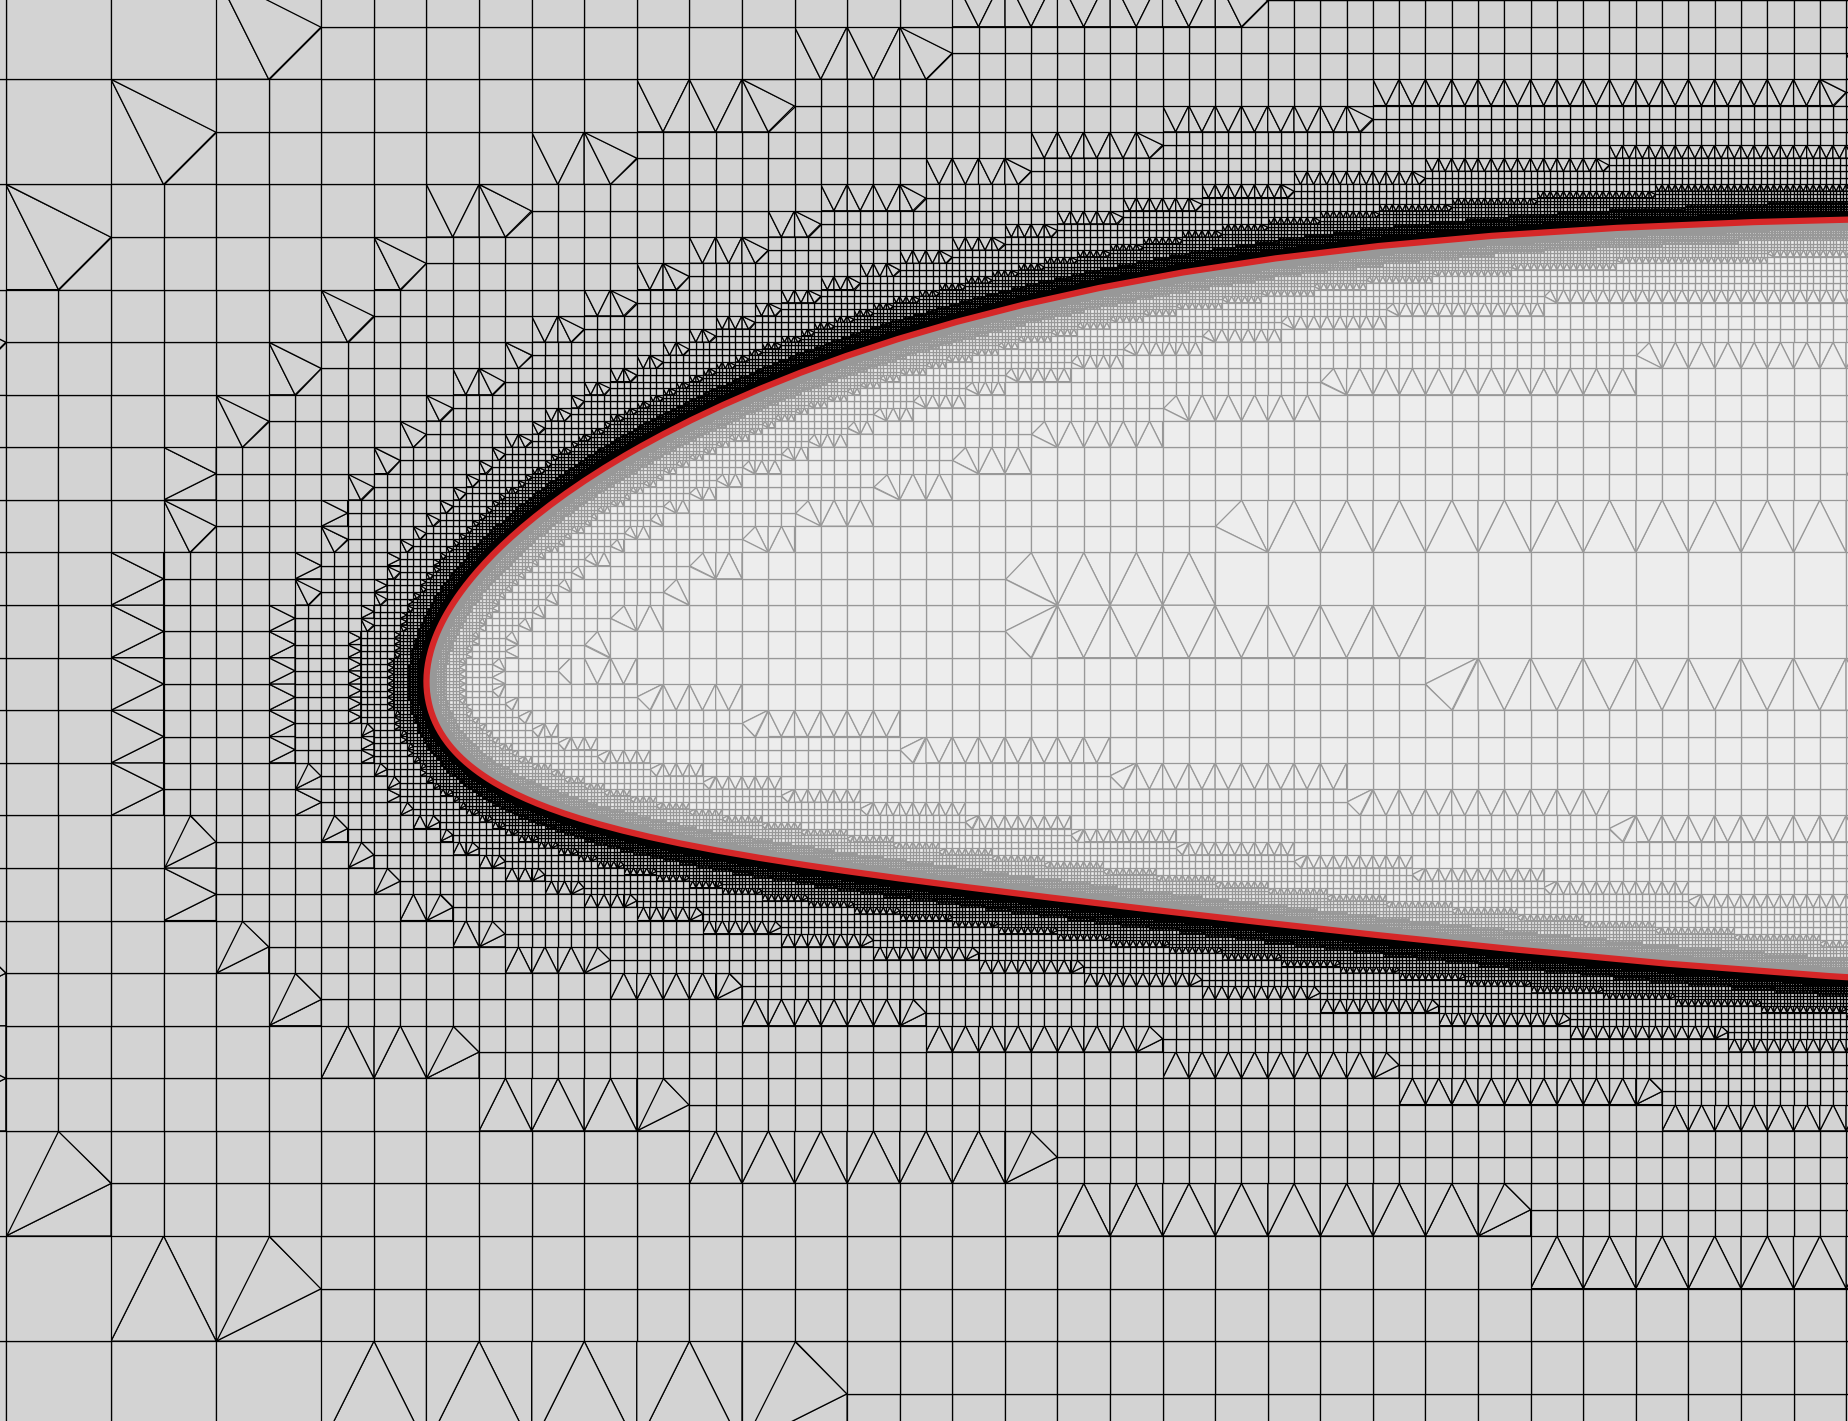
\includegraphics[width=\linewidth,height=2.95cm,keepaspectratio]{FIGURES/INTRODUCTION/meshLE_IBM}}}}%
\only<2>{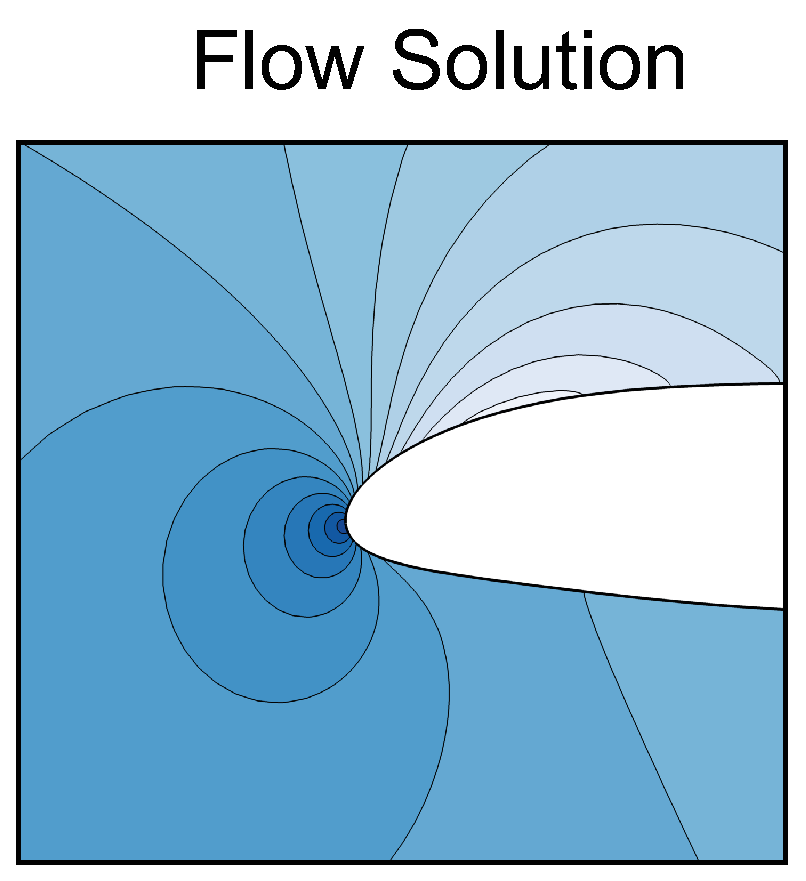
\includegraphics[width=\linewidth,height=4.4cm,keepaspectratio,trim=0 0 0 56,clip]{FIGURES/INTRODUCTION/FLOW}}%
\only<3>{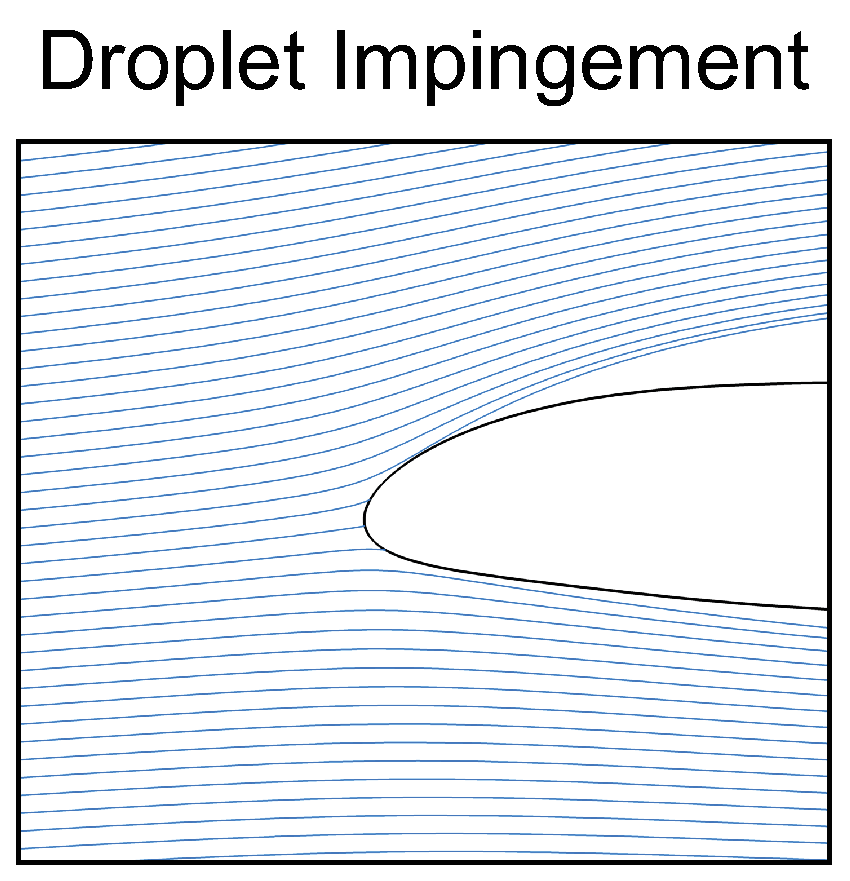
\includegraphics[width=\linewidth,height=4.4cm,keepaspectratio,trim=0 0 0 56,clip]{FIGURES/INTRODUCTION/DROPLET}}%
\only<4>{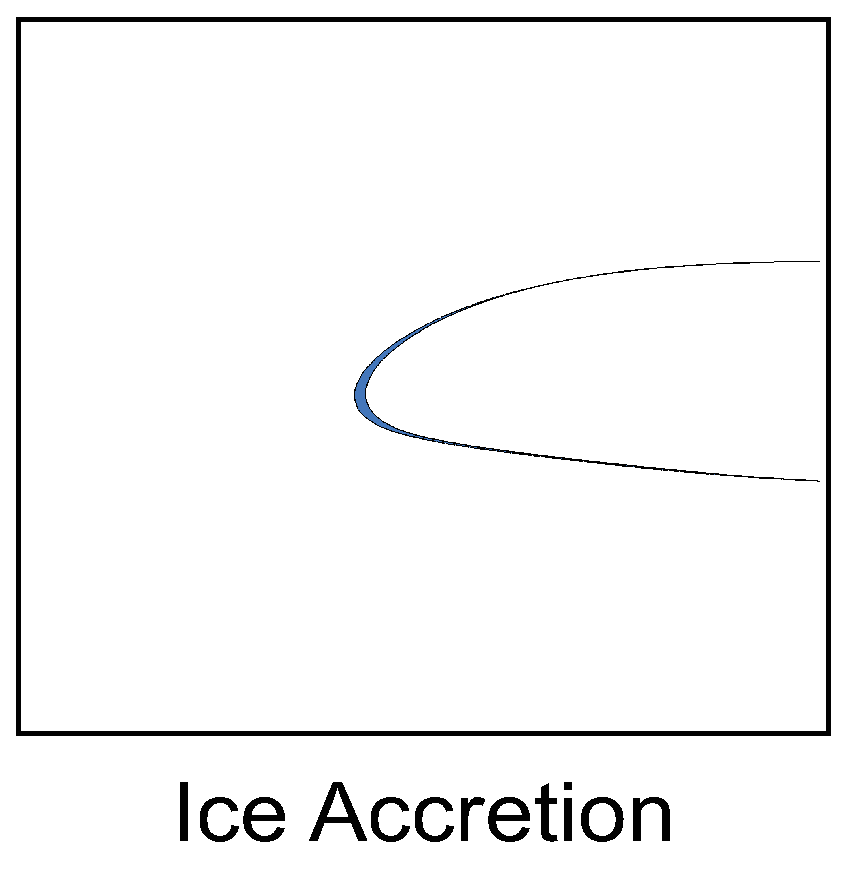
\includegraphics[width=\linewidth,height=4.4cm,keepaspectratio,trim=0 62 0 0,clip]{FIGURES/INTRODUCTION/ACCRETION}}%
\only<5>{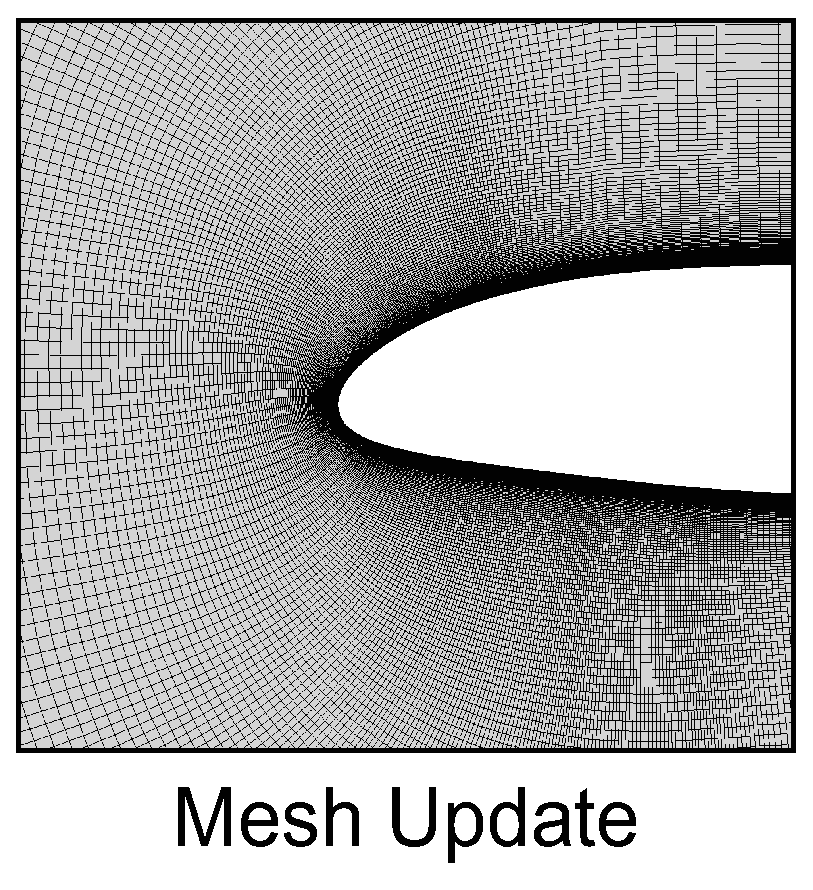
\includegraphics[width=\linewidth,height=4.4cm,keepaspectratio,trim=0 57 0 0,clip]{FIGURES/INTRODUCTION/UPDATE}}%
\end{column}

\end{columns}

\SlideRef{messingerClassical,guardoneReview}
\end{frame}

\begin{frame}{Quasi-Steady Ice-Accretion Framework}
\vspace{-0.15cm}
\begin{center}
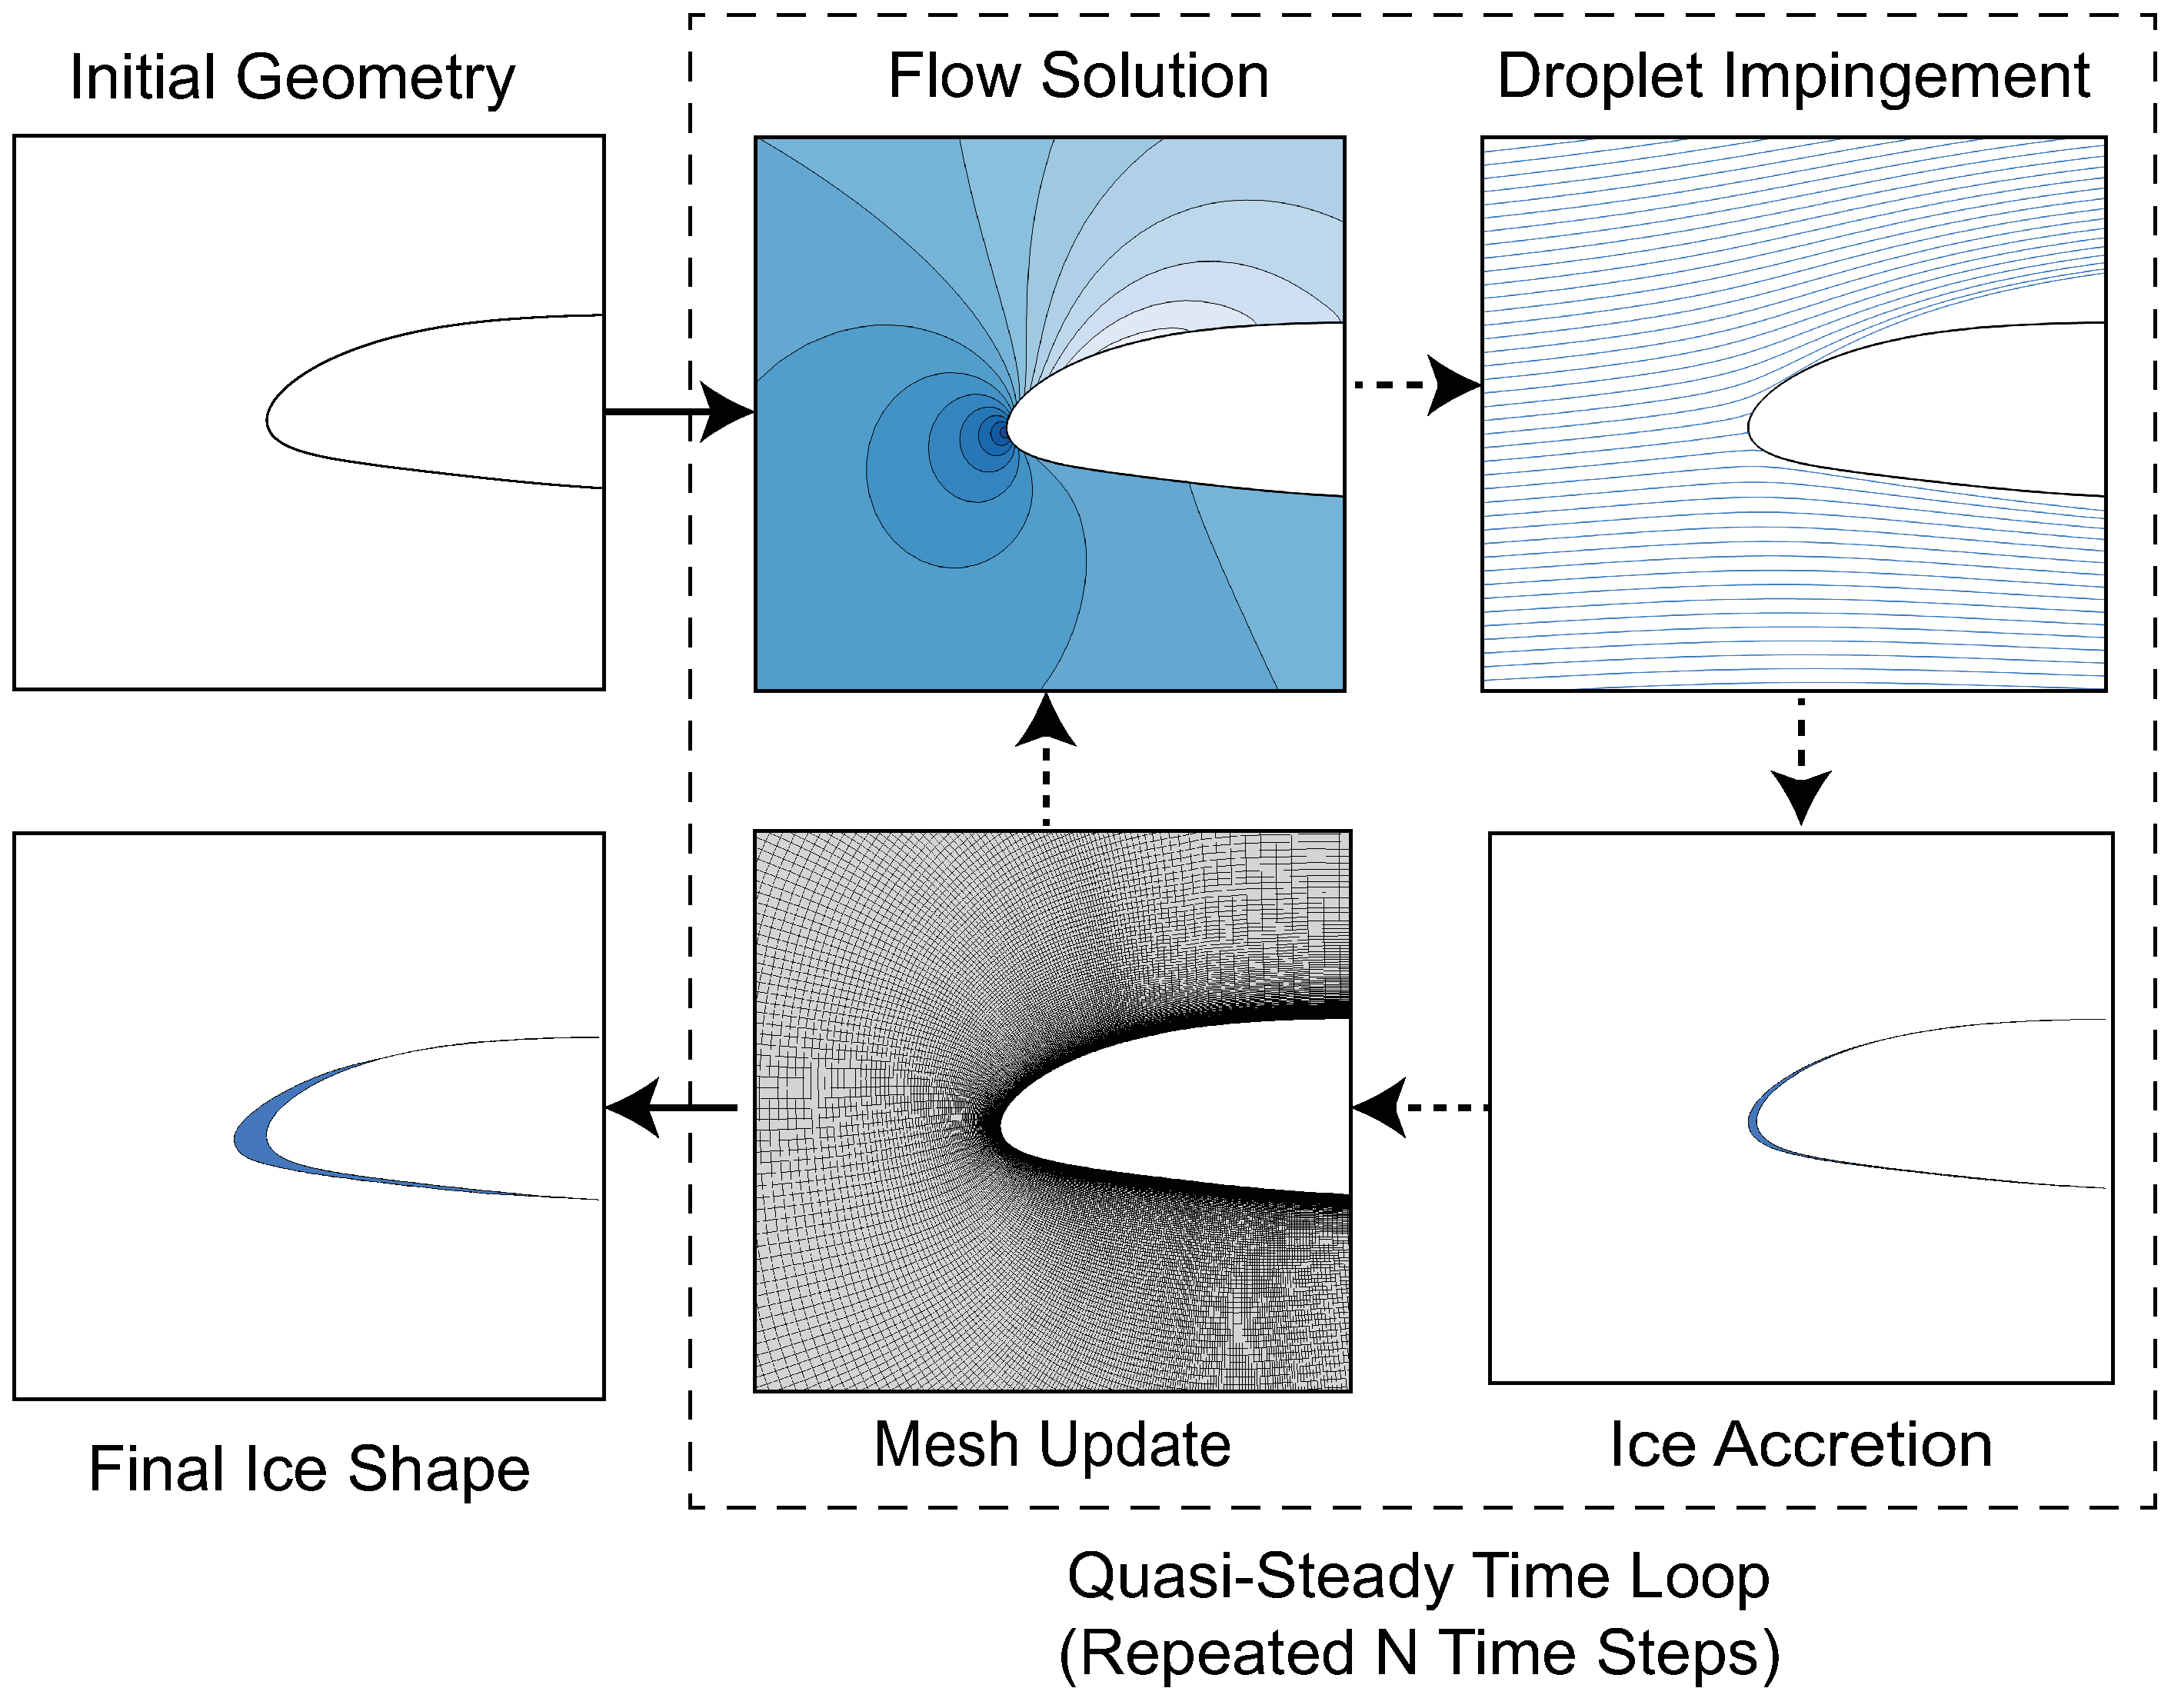
\includegraphics[width=\textwidth,height=0.90\textheight,keepaspectratio]{FIGURES/INTRODUCTION/ICING_FRAMEWORK}
\end{center}
\SlideRef{radenac2024workflow,guardoneReview}
\end{frame}

% ---------------------------------------------------------
% Single-step vs. multilayer ice accretion
% ---------------------------------------------------------
\begin{frame}{Single-Step vs. Multilayer Ice Accretion}
\vspace{0.12cm}
\begin{columns}[T,onlytextwidth]
 \begin{column}{0.485\textwidth}
  \centering
  {\color{champsBlue}\bfseries Single-step ($N=1$)}\par
  \vspace{0.20cm}
  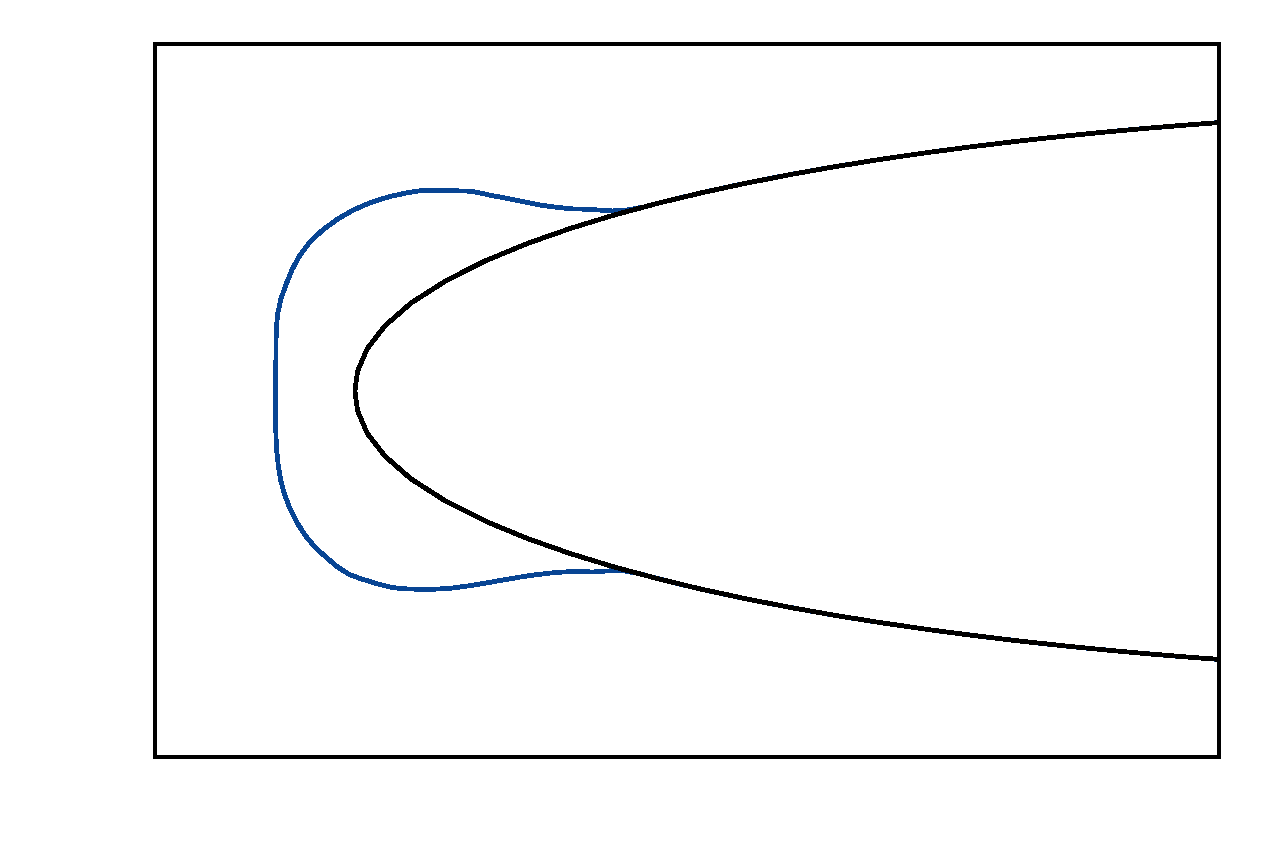
\includegraphics[width=0.98\linewidth,height=3.55cm,keepaspectratio]
    {FIGURES/INTRODUCTION/CASE_362_IPW1_SINGLE_LAYER}\par
  \vspace{0.18cm}
  {\small One accretion interval using the initial aerodynamic and impingement fields.}
 \end{column}
 \begin{column}{0.485\textwidth}
  \centering
  {\color{champsBlue}\bfseries Multilayer ($N=5$)}\par
  \vspace{0.20cm}
  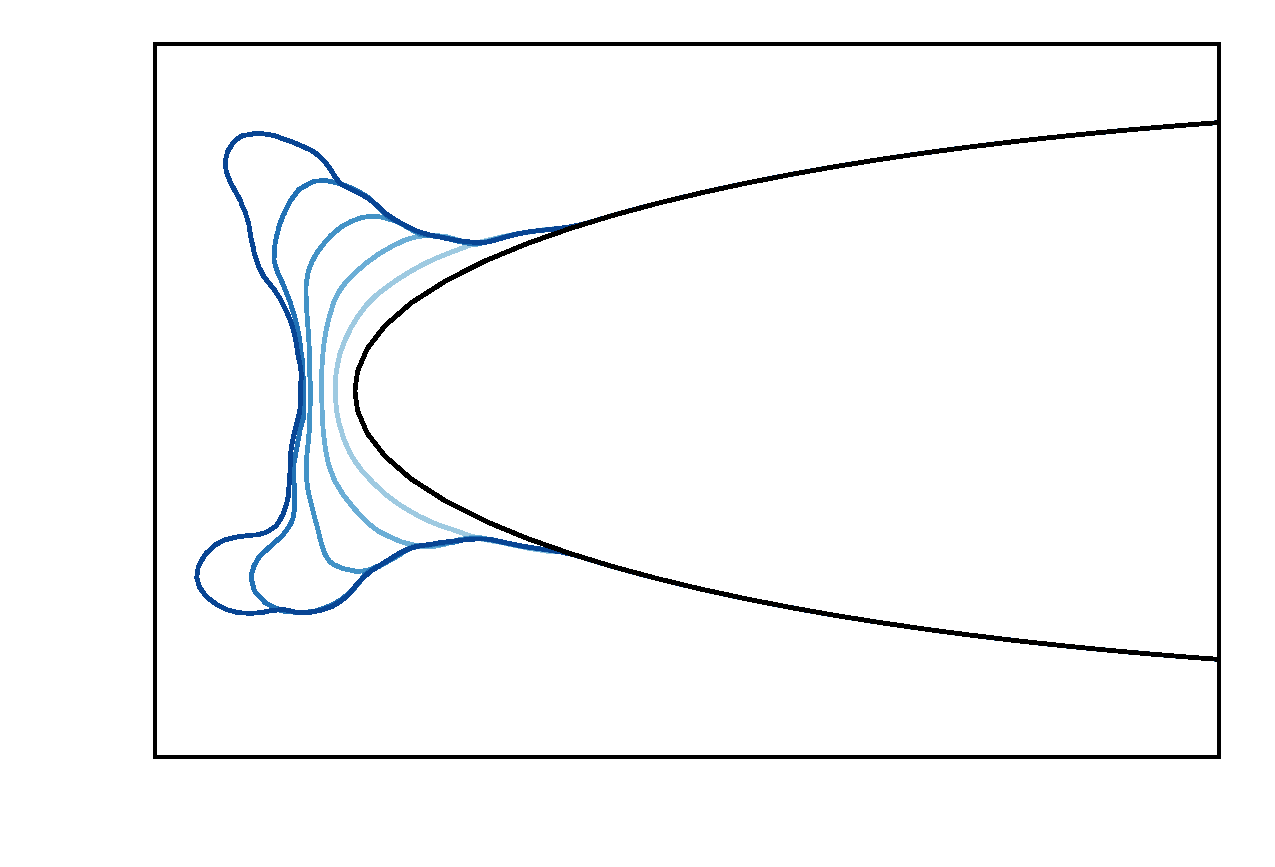
\includegraphics[width=0.98\linewidth,height=3.55cm,keepaspectratio]
    {FIGURES/INTRODUCTION/CASE_362_IPW1_FIVE_LAYERS}\par
  \vspace{0.18cm}
  {\small Repeated geometry updates and recomputation of the coupled fields.}
 \end{column}
\end{columns}
\vfill
\begin{center}
\begin{tikzpicture}
\node[fill=champsBlue!5, draw=champsBlue!18, rounded corners=4pt,
      text width=0.90\textwidth, inner sep=3pt, align=center, font=\small] {%
  \textbf{Geometry feedback matters:} multilayer simulations can capture the development of more complex ice features.};
\end{tikzpicture}
\end{center}
\SlideRef{bourgault-coteMultilayerAirfoilIce2019,radenac2024workflow}
\end{frame}

\begin{frame}{Ice Accretion: Key Terminology}

\vspace{0.15cm}

{\small Ice morphology depends on atmospheric and
aerodynamic conditions and the local freezing process.\par}

\vspace{0.05cm}

\begin{columns}[T,onlytextwidth]

% RIME ICE
\begin{column}{0.315\textwidth}
\centering
{\color{champsBlue}\bfseries\large Rime Ice}

\vspace{0.02cm}

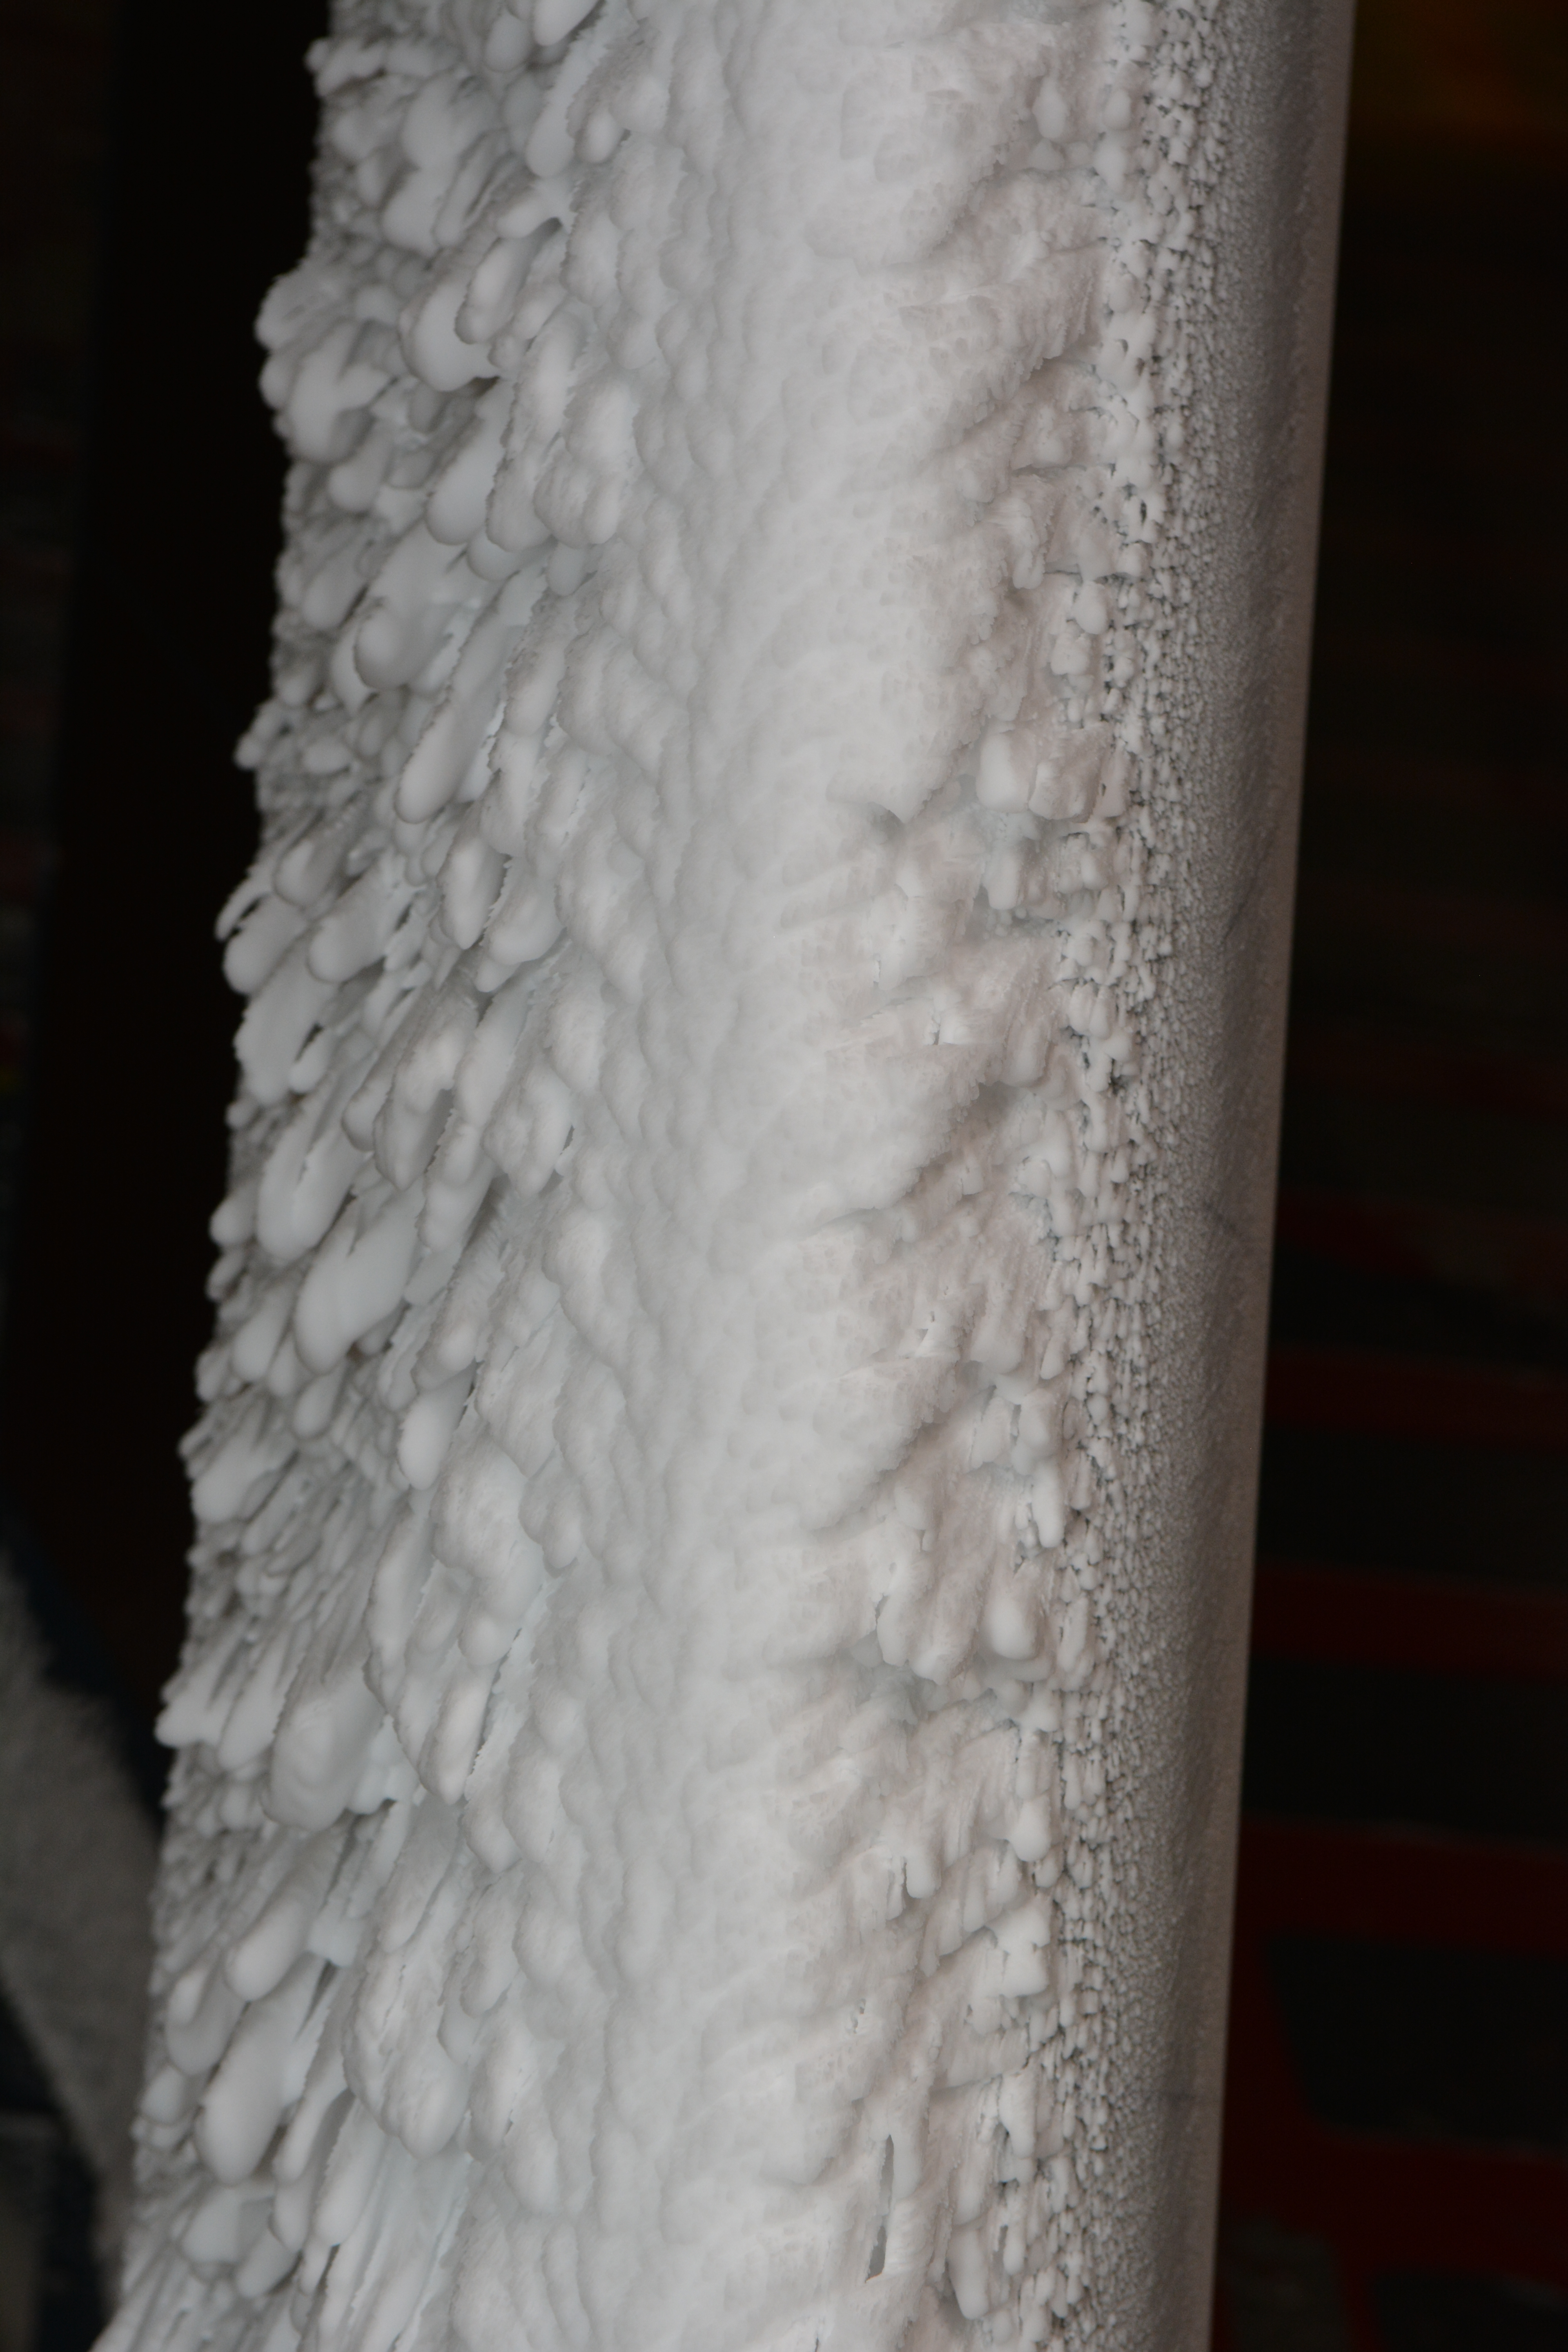
\includegraphics[width=\linewidth,height=3.3cm,keepaspectratio]{FIGURES/INTRODUCTION/CRM_RIME.JPG}

\vspace{0.02cm}

{\footnotesize
Rapid freezing upon impact, producing
streamlined, opaque ice deposits.\par}
\end{column}

% MIXED ICE
\begin{column}{0.315\textwidth}
\centering
{\color{champsBlue}\bfseries\large Mixed Ice}

\vspace{0.02cm}

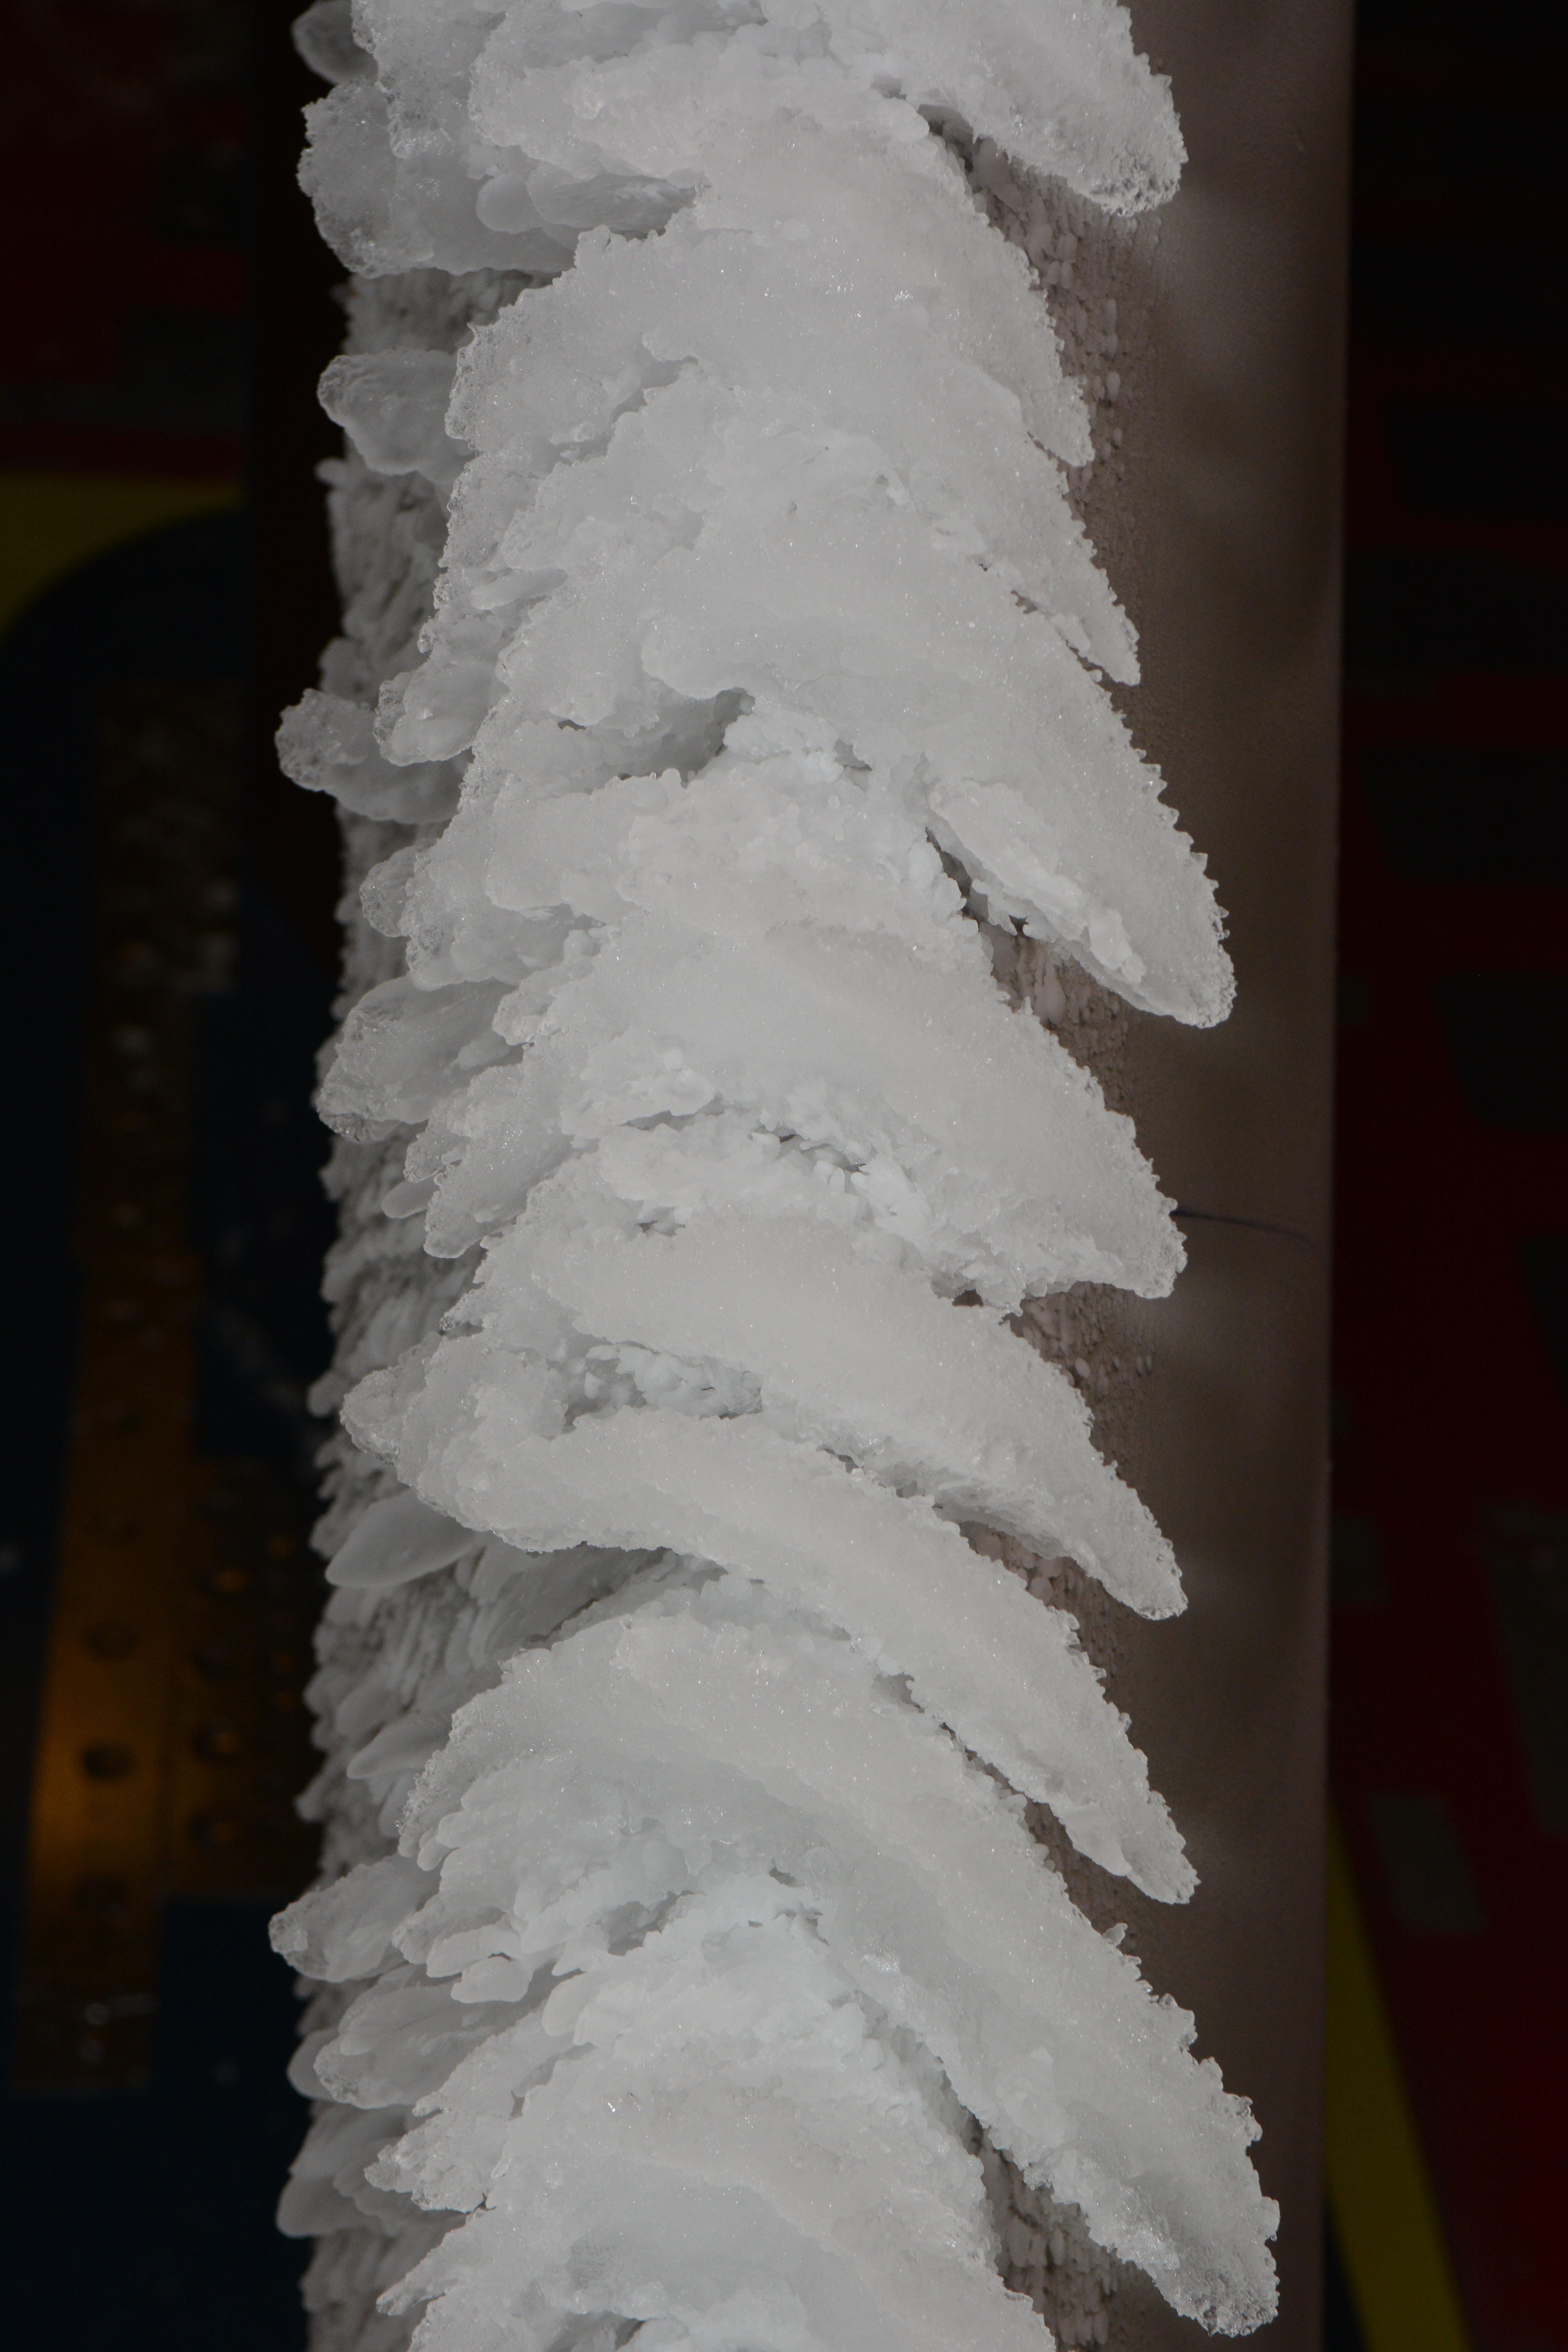
\includegraphics[width=\linewidth,height=3.3cm,keepaspectratio]{FIGURES/INTRODUCTION/CRM_MIXED.JPG}

\vspace{0.02cm}

{\footnotesize
Combination of rime- and glaze-like
ice characteristics.\par}
\end{column}

% GLAZE ICE
\begin{column}{0.315\textwidth}
\centering
{\color{champsBlue}\bfseries\large Glaze Ice}

\vspace{0.02cm}

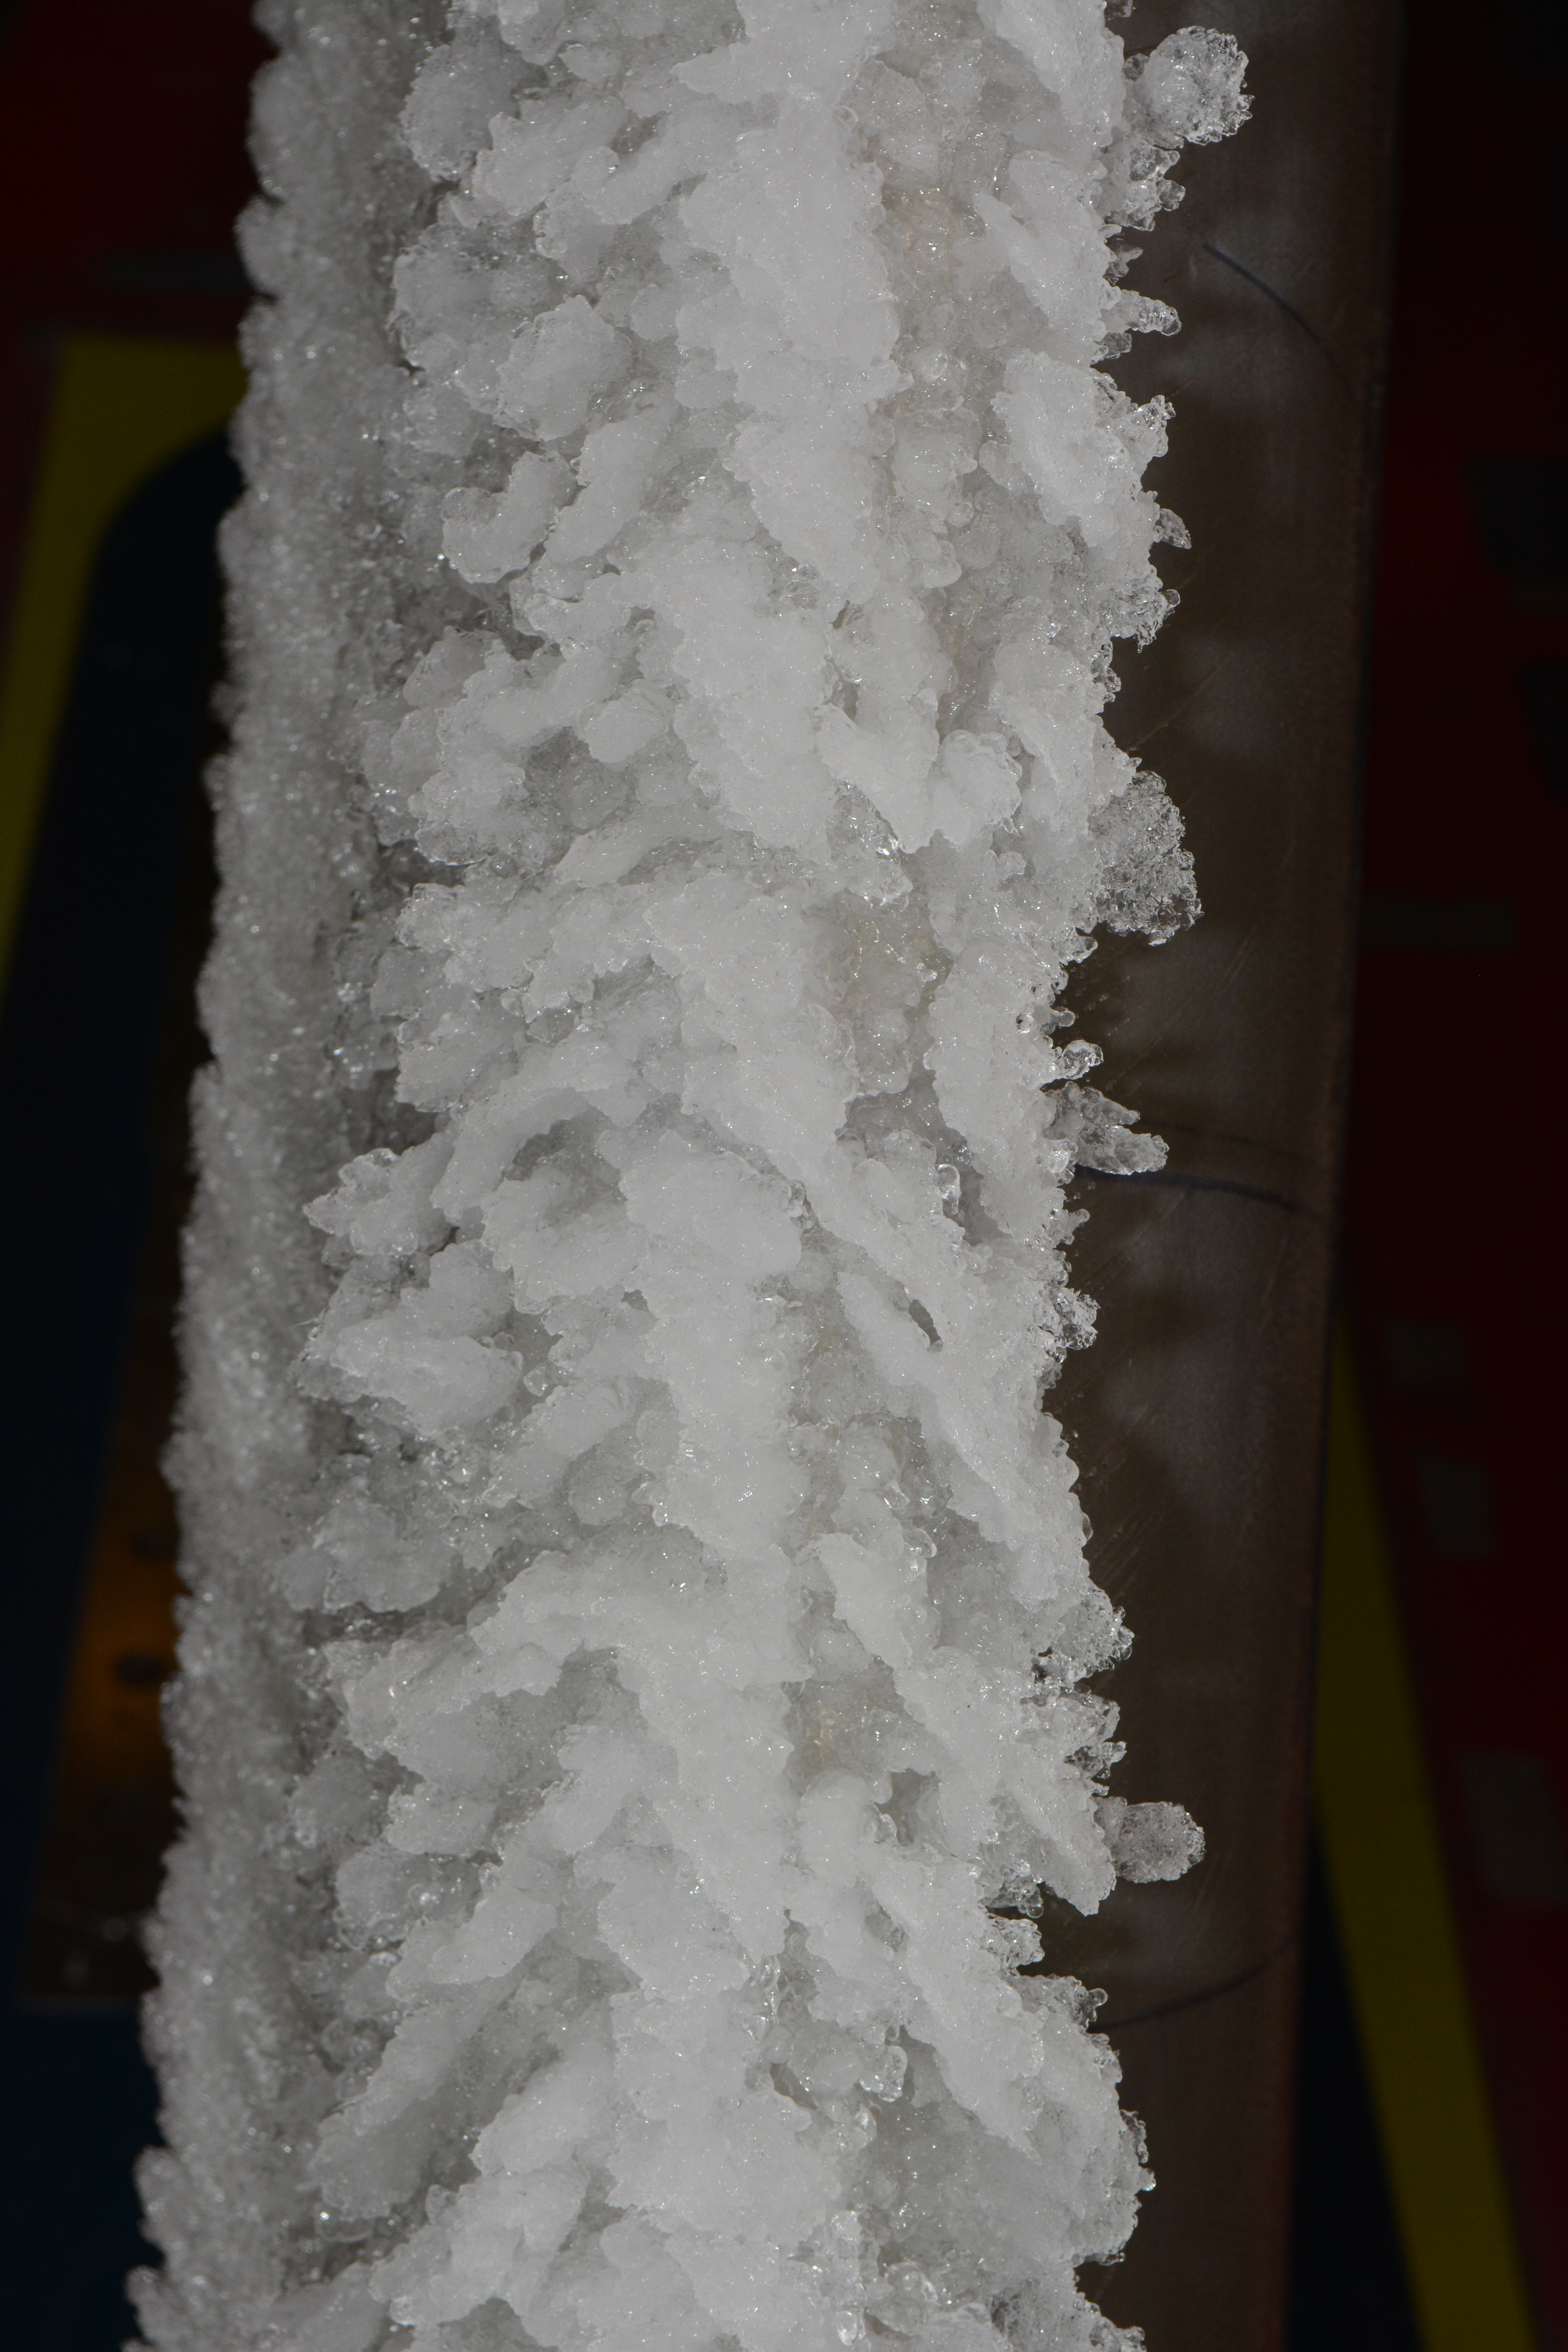
\includegraphics[width=\linewidth,height=3.3cm,keepaspectratio]{FIGURES/INTRODUCTION/CRM_GLAZE.JPG}

\vspace{0.02cm}

{\footnotesize
Partial freezing with liquid-water runback,
often resulting in complex horn-like shapes.\par}
\end{column}

\end{columns}

\vspace{0.15cm}
\noindent\begin{tikzpicture}
\useasboundingbox (0,-0.12) rectangle (\textwidth,0.12);
\shade[left color=blue!70!black, right color=red!80!black]
  (0.16\textwidth,-0.6pt) rectangle (0.83\textwidth,0.6pt);
\fill[red!80!black] (0.83\textwidth,-3pt) -- (0.845\textwidth,0) -- (0.83\textwidth,3pt) -- cycle;
\node[fill=white, inner xsep=4pt, inner ysep=1pt, font=\scriptsize\bfseries, text=champsBlue]
  at (0.5\textwidth,0) {Increasing Ambient Temperature};
\end{tikzpicture}\par
\vspace{0.08cm}

\justifying{\color{champsBlue}\bfseries
Supercooled Large Droplets (SLD):}
{\small
Large droplets that may splash, rebound,
and reimpinge downstream. SLD-related accidents motivated their inclusion
in aircraft certification requirements (Appendix O).\par}

\begin{tikzpicture}[remember picture,overlay]
  \node[anchor=south west,font=\tiny,text=gray]
      at ([xshift=0.1cm,yshift=0.27cm]current page.south west)
      {Images from 2nd Ice Prediction Workshop~\cite{laurendeau2024summary}\quad\cite{FAAAppendixO}};
\end{tikzpicture}

\end{frame}

% ---------------------------------------------------------
% Challenges in 3D multilayer ice accretion
% ---------------------------------------------------------
\begin{frame}{Challenges in Multilayer Ice Accretion}

\vspace{0.1cm}

\begin{columns}[c,onlytextwidth]

% LEFT: challenges, highlighted one at a time
\begin{column}{0.54\textwidth}
\IcingText{01 \quad Droplet Impingement}
{Lagrangian tracking naturally captures individual
droplet dynamics and enables SLD modeling.
\textbf{How can it remain efficient and scalable
for complex 3D configurations?}}
\par\vspace{0.2cm}

\IcingText{02 \quad Geometry Evolution}
{Direct surface-node displacement can lead to
mesh degradation and entanglement.
\textbf{How can complex 3D ice geometries be evolved
robustly over successive accretion layers?}}
\par\vspace{0.2cm}

\IcingText{03 \quad Geometry Representation}
{Body-fitted approaches require repeated
flow-mesh deformation or remeshing.
\textbf{How can immersed-boundary methods reduce
these constraints while achieving comparable accuracy?}}
\end{column}

% RIGHT: one illustration per challenge
\begin{column}{0.43\textwidth}
\centering
\parbox[c][6.6cm][c]{\linewidth}{\centering
\only<1>{%
  {\scriptsize\color{champsBlue}\bfseries Lagrangian droplet tracking}\par\vspace{0.05cm}
  \movie[width=\linewidth,height=0.5625\linewidth,poster,showcontrols,loop,autostart]%
    {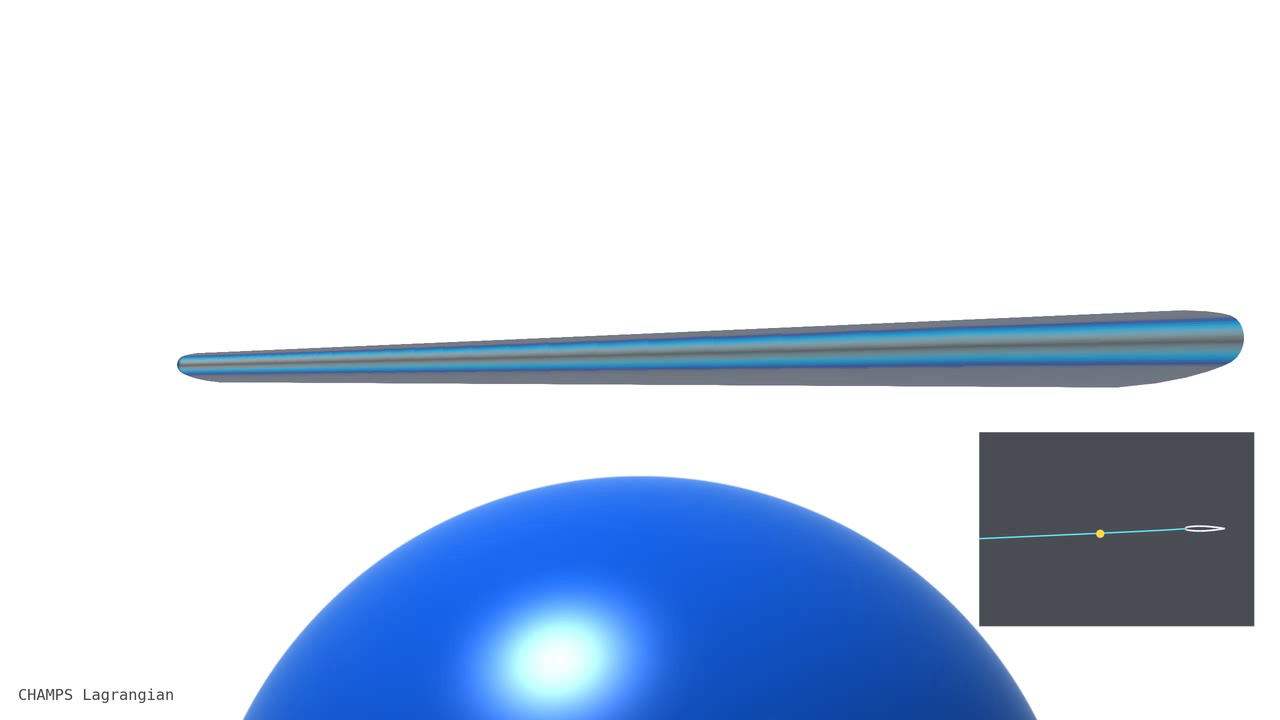
\includegraphics[width=\linewidth]{FIGURES/INTRODUCTION/DROPLET_POV_poster.png}}%
    {FIGURES/INTRODUCTION/DROPLET_POV.mp4}}%
  %{\tiny\itshape\color{gray}POV: You're a supercooled water droplet approaching an aircraft wing.\\No water droplet was harmed making the video.\par}}%
\only<2>{%
  {\scriptsize\color{champsBlue}\bfseries Direct surface-node displacement}\par\vspace{0.05cm}
  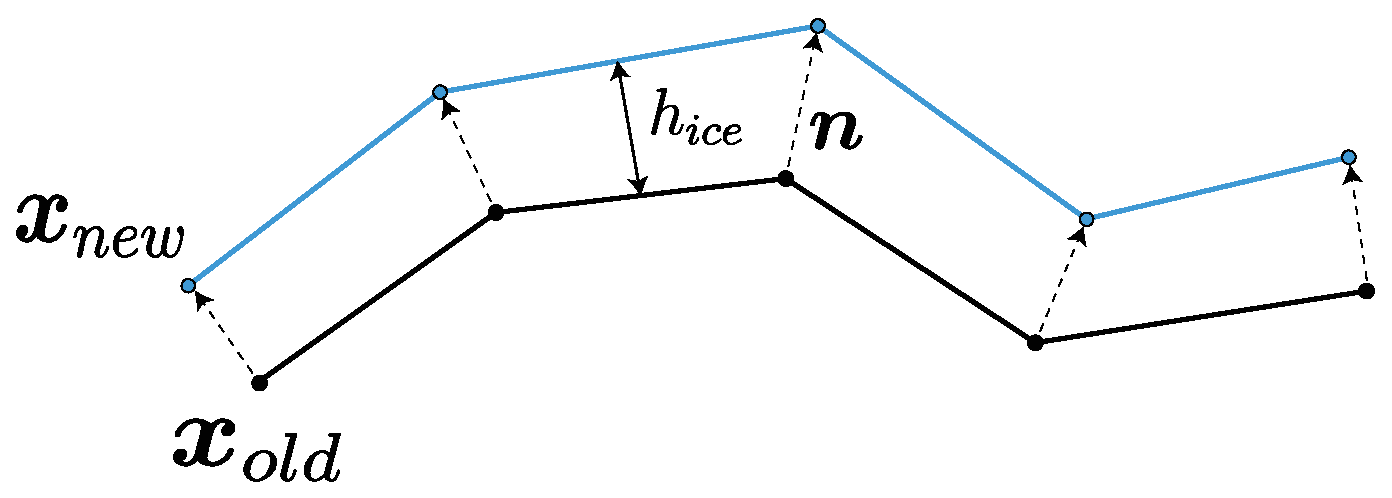
\includegraphics[width=\linewidth,height=2.1cm,keepaspectratio]{FIGURES/INTRODUCTION/LAGRANGIAN_NODE_DISPLACEMENT}\par
  {\small$\mathbf{x}_{\mathrm{new}}=\mathbf{x}_{\mathrm{old}}+h_{\mathrm{ice}}\,\mathbf{n}$}\par\vspace{0.04cm}
  {\scriptsize\color{champsBlue}\bfseries Increasing geometric complexity}\par\vspace{0.05cm}
  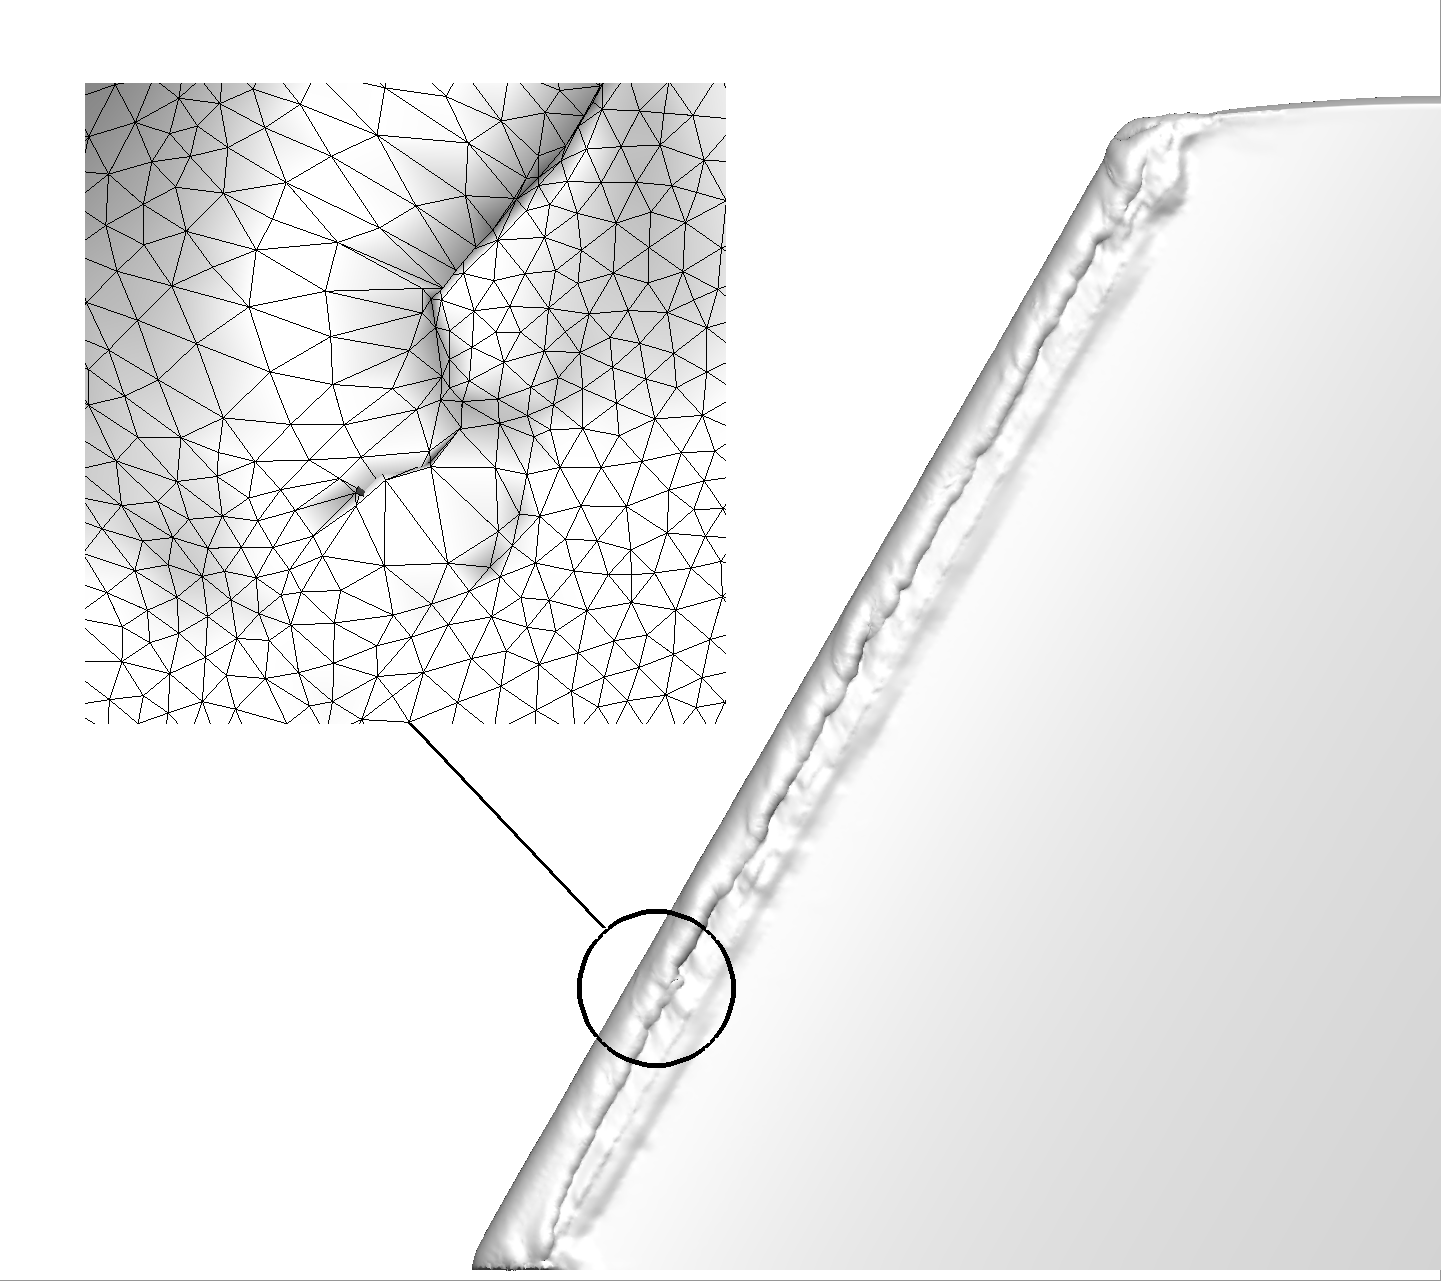
\includegraphics[width=\linewidth,height=3.75cm,keepaspectratio]{FIGURES/INTRODUCTION/ENTANGLEMENT.png}}%
\only<3>{%
  {\scriptsize\color{champsBlue}\bfseries Immersed boundary}\par\vspace{0.05cm}
  {\setlength{\fboxsep}{0pt}\setlength{\fboxrule}{0.6pt}\fbox{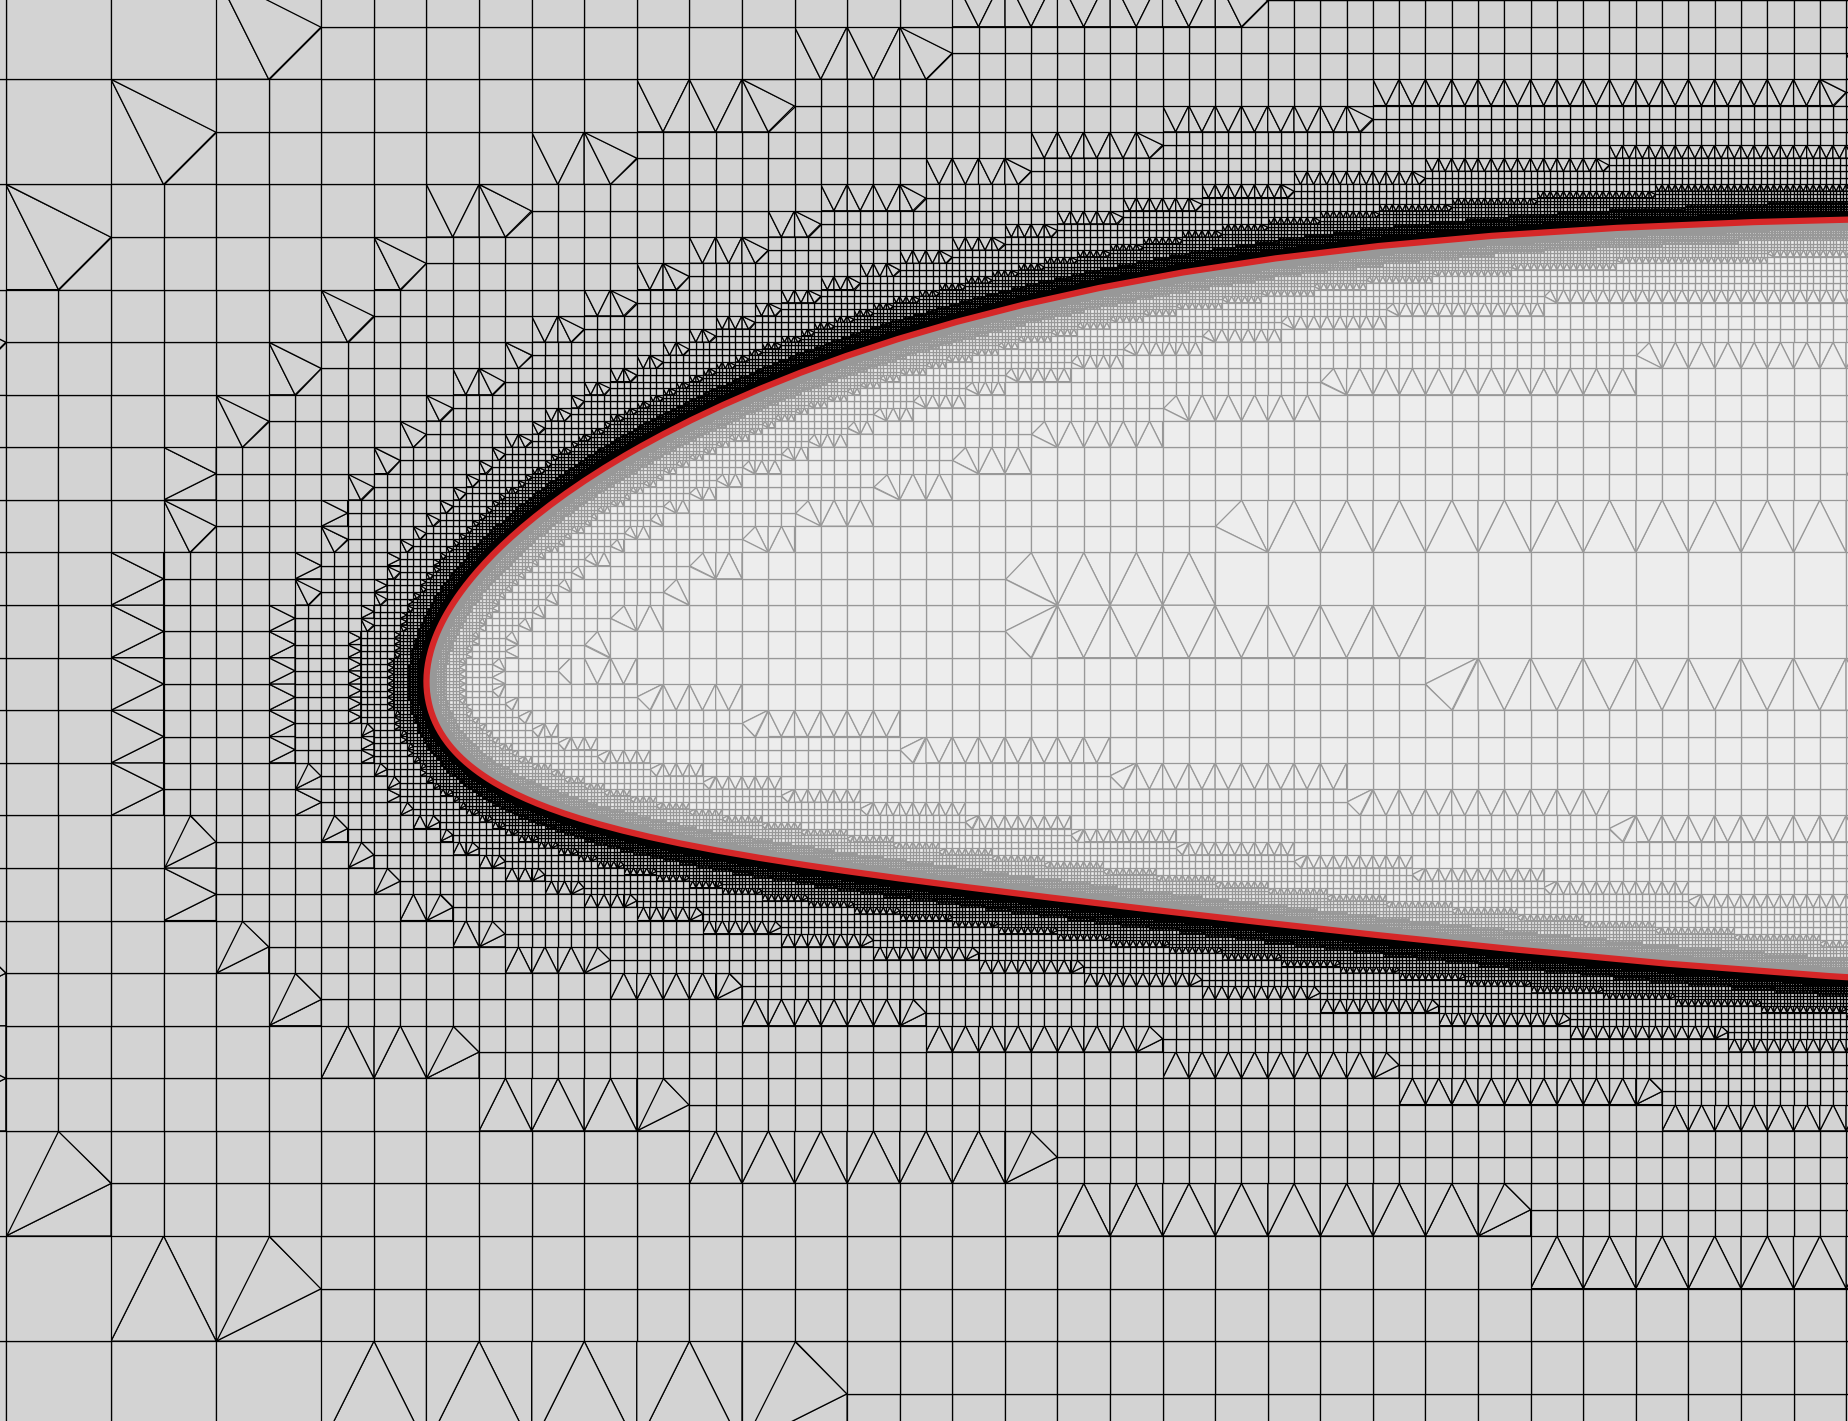
\includegraphics[width=\linewidth,height=4.5cm,keepaspectratio]{FIGURES/INTRODUCTION/meshLE_IBM}}}}%
}
\end{column}

\end{columns}

\SlideRef{lagNodeDisplacement,thompsonDeformation,lavoie2021immersed}
\end{frame}

\begin{frame}{Research Objectives}

\vspace{0.12cm}

% OVERALL OBJECTIVE
\begin{center}
\begin{tikzpicture}
\node[
    fill=champsBlue!7,
    rounded corners=4pt,
    text width=0.90\textwidth,
    inner sep=0.25cm,
    align=center
] {
    {\color{champsBlue}\bfseries Overall Objective}\\[0.12cm]
    Improve the \textbf{robustness and efficiency of
    three-dimensional multilayer ice-accretion simulations},
    with an emphasis on complex geometry evolution.
};
\end{tikzpicture}
\end{center}

\vspace{0.30cm}

% THREE CONTRIBUTIONS
\IcingText{01 \quad Lagrangian Droplet Impingement}
{Develop efficient and scalable Lagrangian tracking
methods for complex 3D configurations,
including SLD effects.}

\par\vspace{0.28cm}

\IcingText{02 \quad Three-Dimensional Level-Set Ice Accretion}
{Develop a robust approach for multilayer
geometry evolution and surface reconstruction,
avoiding mesh entanglement.}

\par\vspace{0.28cm}

\IcingText{03 \quad Immersed Boundary Method}
{Extend the existing immersed-boundary flow solver
to enable coupled ice-accretion simulations while
reducing repeated body-fitted aerodynamic remeshing.}

\end{frame}

% Add section slides here.
